\documentclass[10pt,twocolumn]{article}
\usepackage{usenix}
\usepackage{epsfig}
\usepackage{endnotes}
\usepackage{amsfonts}
\usepackage{mathrsfs}
\usepackage{balance}
\usepackage{hyperref}
\usepackage{algorithm2e}
\usepackage{amsmath}
\usepackage{amssymb}
\usepackage{amsthm}
\usepackage{mathtools}
\usepackage{courier}
\usepackage{tabularx}
\usepackage{subfig}
\usepackage{textcomp}
\usepackage[OT1]{fontenc}
\usepackage{xcolor}
\usepackage[miktex]{gnuplottex}
\usepackage[labelfont=bf]{caption}
\hypersetup{
    colorlinks,
    linkcolor={red!50!black},
    citecolor={blue!50!black},
    urlcolor={blue!80!black}
}


\newcommand{\sys}{{\textsc{SocksDirect}}\xspace}
\newcommand{\libipc}{{\textsc{libsd}}\xspace}
\newcommand{\RED}[1]{\textcolor[rgb]{1,0,0}{#1}}
\newcommand{\paraspace}{\vspace{0.05in}}
\newcommand{\parab}[1]{\paraspace\noindent{\textbf{#1}}}
\usepackage[normalem]{ulem}
\usepackage{eucal}
\usepackage{pifont}
\newcommand{\yes}{\ding{51}}

\graphicspath{{figure/}}

%
% import the customized commands
%

\begin{document}

%\title{SocksDirect: Push-Button Acceleration of Linux Socket~\vspace{-0.1in}}
\title{SocksDirect: Fast and Compatible Socket in User Space~\vspace{-0.1in}}

\author{{\rm OSDI'18 Submission \#264}\vspace{-0.5in}}

\newcommand{\authornote}[1]{\raisebox{0.8ex}{$#1$}}
\maketitle

\newcommand{\specialcell}[2][c]{%
  \begin{tabular}[#1]{@{}c@{}}#2\end{tabular}}


\section*{Abstract}

Linux socket is implemented in the kernel space with shared data structures that needs concurrency protection, which incurs significant overhead.
Communication intensive applications in hosts with multi-core CPU and high-speed networking hardware often put considerable stress on the socket system.
Recent work on user-space sockets either does not support intra-host communication among containers and applications, or has limitations on compatibility, isolation and multi-thread scalability.
%Communication intensive applications on modern computers with multi-core CPU and high-speed networking hardware 
%often put considerable stress on traditional socket implementation. 
%This design incurs significant kernel crossing and locking overhead.
%Recent user-space sockets often do not support intra-host communication among containers and applications, or have limitations on compatibility, isolation and scalability with multiple threads and concurrent connections.

%In this paper, we describe \sys{}, a high performance socket system that is fully compatible with Linux and can be used as a drop-in replacement with no modification to applications.
%\sys{} is implemented in user space to avoid kernel crossing cost and simplify deployment.
%Each host runs a monitor daemon to securely process the control plane, while the data plane bypasses the monitor.
%We achieve multi-thread scalability by considering threads as a shared-nothing message passing distributed system.
%To improve memory locality, we multiplex all connections and event notifications between a pair of threads via one queue.
%We use a high performance shared memory queue for intra-host communication.
%For inter-host communication, we take advantage of modern RDMA hardware, but can also transparently communicate with regular TCP/IP endpoints.
%Together with carefully designed zero-copy mechanism and cooperative multitasking, it removes many overheads of existing socket systems.
%Experiment shows that \sys{} achieves 4 to 24x message throughput, 10 to 60x better latency, and over 40x connection setup throughput compared with Linux socket.


In this paper, we describe \sys{}, a high performance socket system. \sys{} is implemented in user space to avoid kernel crossing cost. 
It achieves security and isolation by employing a trusted monitor daemon to handle control plane operations such as connection establishment and access control. 
\sys{} is fully compatible with Linux socket and can be used as a drop-in replacement with no modification to existing applications. The design fully
handles Linux fork semantics, and can handle both intra- and inter-host communications with hosts equipped with \sys{} as well as those without. 
Last but not least, \sys{} is performant. \sys{} uses shared memory queue and modern RDMA transport for intra- and inter-host communication.
It removes multi-thread synchronization in common cases and improves memory efficiency with many concurrent connections.
It leverages techniques such as cooperative multitasking and page-remapping based zero-copy to remove many overheads of existing socket systems.
Experiment shows that \sys achieves 7 to 20x better message throughput, 17 to 35x better latency, and 20x connection setup throughput compared with Linux socket.


\section{Introduction}
\label{sec:intro}

%Most cloud applications use the socket API for inter-process communication among components or containers inside a same server and across data center network, in addition to serving Internet users. For example, communication intensive applications (\textit{e.g.} nginx and memcached) spend 50\%$\sim$90\% of CPU time in the OS kernel, mostly processing socket operations.
%The overhead of Linux socket attributes to kernel crossing in system calls, context switch, process scheduling, synchronization, memory copy, cache miss and TCP transport.
%Applications in high performance computing have a long tradition of using shared memory for intra-server communication and RDMA for inter-server, thus avoiding the overheads above.
%However, these abstractions are radically different from socket, so it is complicated and potentially insecure to port socket applications to shared memory and RDMA.
%The overhead of Linux socket becomes salient given the rapid growth of network speed and number of CPU cores per server. %We benchmark communication intensive applications (\textit{e.g.} Nginx and memcached) and find that 50\%$\sim$90\% of CPU time is spent in the OS kernel. When more CPU cores are utilized, they even spend a larger portion of time in the kernel~\cite{boyd2010analysis}. In addition to CPU overhead, latency is also a problem. The round-trip time (RTT) between two processes communicating with shared memory can be as low as 0.2$\mu$s, while TCP socket RTT between two cores is $\approx$16$\mu$s. In a data center, the RTT between RDMA servers is also one order of magnitude lower than kernel TCP/IP stack.

Socket API is the most widely used communication primitive, and is the fundamental building block for inter-process communication. Traditional Linux socket is expensive. Communication intensive applications could spend 50\%$\sim$90\% of CPU time in the OS kernel, mostly processing socket operations. There has been extensive work aiming at reducing the socket overhead~\cite{peter2016arrakis,yasukata2016stackmap,nishtala2013scaling}. These approaches still has limitations, either not fully removing some of the important overheads such as context switch and synchronization~\cite{lin2016scalable,han2012megapipe,jeong2014mtcp,baumann2009multikernel}, not fully compatible with Linux socket API~\cite{}, or cannot take advantage of modern networking hardware capabilities such as RDMA~\cite{dunkels2001design,jeong2014mtcp,libvma,openonload}. A comparison of \sys with existing work is discussed in more detail in Sec.\ref{sec:related}.
%There has been extensive work aiming to release the bare metal performance of multi-core CPU and data center network. For intra-server communication, there are mainly three lines of research. The first category of work use the NIC as a switch~\cite{peter2016arrakis,belay2017ix,yasukata2016stackmap}, but going deep to the NIC introduces $\approx2 \mu$s delay due to PCIe latency, one order of magnitude higher than shared memory. A second line of work optimize or redesign the kernel socket stack~\cite{lin2016scalable,han2012megapipe,jeong2014mtcp,baumann2009multikernel}, where the kernel uses peer-to-peer shared memory communication among cores. However, this approach does not eliminate context switch overhead, while system call batching introduces extra latency. Some other works use dedicated cores as a virtual switch~\cite{huang2017high}, which limits multi-core scalability.

%For inter-server communication, most works leverage a user-space stack~\cite{dunkels2001design,jeong2014mtcp,libvma,openonload} to achieve kernel bypass, but the CPU still needs to handle reliable transport. As RDMA becomes widely available in data centers, we hope to offload the transport to RDMA NICs when the peer supports RDMA. Furthermore, most works assume only one connection per pair of processes. However, load balancers, web servers and application gateways serve many concurrent connections~\cite{nishtala2013scaling,lin2016scalable,belay2017ix}. In light of this, both connection setup, event notification and data transmission under high concurrency need to be efficient.

%To demonstrate high performance, most existing works propose new abstractions for inter-process and inter-server communication.  existing socket applications need modifications to use the new abstractions. Furthermore, these stacks are not optimized for a large number of concurrent or short-lived connections, which is an important workload to serve Internet users and large distributed systems.

%One line of research optimize the kernel code or design user-space compatible stacks for higher socket performance. The kernel optimization approach does not eliminate context switch overhead, while system call batching introduces extra latency. User-space stacks are mostly designed for inter-server connections. With the trend of containerized micro-services, we expect an increasing number of applications or containers to be hosted on each server, where inter-process communication (IPC) inside server has more significance.

%To simplify deployment, we hope to accelerate existing applications without modification to the code. \textit{Socket compatibility} adds another dimension of challenge. The socket interface was designed for networking and IPC in millisecond scale, when memory copy, context switch, synchronization, cache miss and cache migration were considered inexpensive~\cite{barroso2017attack,belay2017ix}. An efficient socket architecture for microsecond-scale networking and IPC requires minimizing all overheads above. The semantics lead to challenges. First, the send buffer can be modified by application after non-blocking \texttt{send}, and the receive buffer is not determined until application calls \texttt{recv}. Data copy on \texttt{send} and \texttt{recv} seems mandatory. Second, connections are shared by processes and threads after \texttt{fork} and thread creation. It is challenging to avoid synchronization in this multi-producer and multi-consumer FIFO model. Third, multiple processes listening on a same IP and port compete for incoming connections.

%\textbf{The above part is motivation and related work.}

We design \sys{}, a high performance user-space socket architecture that is compatible with existing applications and preserves isolation among processes, while being scalable to multiple cores and many concurrent connections. The main component of \sys{} is a user-space library \libipc{} that intercepts and implements Linux socket APIs. User application can take advantage of \libipc by simply using the \textit{LD\_PRELOAD} environment variable in Linux to load the library, and the library can intercept the system call wrappers of GNU libc. 



\sys is designed to be compatible with existing applications using Linux socket. Therefore, it preserves Linux socket semantics, and in particular it behaves correctly with fork and thread creation. \textit{Process isolation} also needs to be preserved in \sys.
%\parab{User-mode socket library as a drop-in replacement.}

\sys is designed to fully support efficient intra-server and inter-server communications. For inter-process connections within a single server, we use peer-to-peer shared memory in user space without going deep into the kernel or NIC. For communication between nodes in an RDMA enabled data center, we offload the transport to RDMA NICs. Finally, we use a lightweight user-space TCP/IP stack~\cite{dunkels2001design} to communicate with hosts without RDMA support.

%The emergence of containers and micro-services draws attention to intra-server communication~\cite{bailis2016introducing}.
%%For manageability and fault isolation, developers break monolithic services into self-contained microservice containers, interconnected via container network. 
%Following the trend of recent data-plane operating systems~\cite{peter2016arrakis,belay2017ix,freeflow}, 
%\sys should optimize for both intra-server and inter-server socket.

We set out to build \sys{} to have very high performance. To this end, \sys has four performance goals. The first two are \textit{low latency} and \textit{high throughput} (aka low CPU overhead). For inter-process connections within a server, the latency and throughput should be comparable with shared memory communication. For inter-server connections in a data center, we aim at performance close to raw RDMA. Moreover, performance should be \textit{scalable} to be able to leverage multiple cores. Finally, the performance should not degrade with large number of \textit{concurrent connections} between two processes. 
% Many user connections are forwarded from the load balancer to an application~\cite{lin2016scalable}. Some applications create a TCP socket to key-value store for each request they process~\cite{nishtala2013scaling}.

The key to multi-core scalability and inter-process isolation is to avoid synchronization and state sharing. We \textit{consider processes as a distributed system} that communicates via message passing. To avoid synchronization among threads, each thread is regarded as a separate process. We further partitioning socket states to each process and implement the socket APIs \textit{as local to the process as possible}. 
%To maximize message passing performance, we design a high performance queue between each pair of processes, thus avoiding synchronization and atomic operations. The queue uses shared memory ring buffer inside a server and one-sided RDMA \texttt{write} across data center network.

%We further minimize message passing by partitioning socket states to each process. We implement the socket APIs \textit{as locally as possible}. In particular, we allocate file descriptors, buffers and manage socket options in the caller process. For non-local operations, we make the best effort to \textit{minimize centralized coordination and blocking wait}. Data transmission and event multiplexing operations (\textit{e.g.} \texttt{send}, \texttt{recv} and \texttt{epoll}) only need non-blocking access to peer-to-peer communication channels. For connection establishment, each server has a coordinator process, called \textit{monitor}, to load balance incoming connections, setup inter-process queues and enforce ACL policies. Delegation to the monitor is more secure and efficient than inter-process synchronization~\cite{roghanchi2017ffwd}.


To handle many concurrent connections efficiently, we need to save memory footprint and improve locality of memory accesses. Observing the event-driven behavior of applications, we use cooperative multitasking to minimize kernel event processing overhead. For each pair of processes, we \textit{multiplex socket connections through one queue}, so sending a small message involves only one cache migration or RDMA write (amortized).

%The POSIX socket API was designed for networking and IPC in millisecond scale, leading to two performance challenges. First, connections are shared by processes and threads after \texttt{fork} and thread creation. Linux protects this multi-producer multi-consumer FIFO with locks. To scale a shared socket, we \textit{optimize for the common case and prepare for the worst case}. Senders transmit data via different queues in parallel. To ensure receiver ordering, based on the observation that applications seldom receive concurrently from a shared socket, the sender designates a receiver with exclusive access. We further develop mechanisms to avoid deadlock and starvation, in addition to handling unconsumed buffers during \texttt{fork} and thread creation.

%Second, the send buffer can be modified by application after \texttt{send}, and the receive buffer is not determined until application calls \texttt{recv}. Data copy on \texttt{send} and \texttt{recv} seems mandatory. To avoid memory copy of large buffers, we extend the \textit{page remapping} approach~\cite{thadani1995efficient,chu1996zero}, which enables copy-on-write upon \texttt{send} and remaps send buffer to receiver's virtual address upon \texttt{recv}.
%First, we intercept \texttt{memcpy} of full pages to reduce copy-on-write. Second, we move kernel-based page allocation to user-space while preserving security.
%As a result, we achieve zero copy for both shared memory, RDMA and TCP transport.

\RED{Simplify evaluation.}

On the latency side, \sys{} achieves $0.25\mu$s RTT for intra-server socket, 60x faster than native Linux Sockets and only $0.05\mu$s higher than a bare-metal shared memory queue. For inter-server socket, \sys{} achieves $2\mu$s RTT between RDMA hosts, almost the same as raw RDMA verbs and reduces Linux RTT by 10x. The RTT to a TCP/IP peer is $5\mu$s. On the throughput side, every second, a single-thread process can send 11~M intra-server messages (4x Linux), 8~M messages via RDMA (24x Linux) or 5~M messages via TCP/IP (15x Linux). Each thread can establish up to 1~M new connections per second (40x Linux). It is worth noting that the throughput is scalable with number of cores and connections.

We evaluate end-to-end performance of \sys{} using two categories of applications: \textit{network functions} and \textit{web services}. For a multi-core pipelined network function chain, a socket application accelerated by \sys{} achieves comparable performance as a state-of-the-art framework specialized for network functions~\cite{panda2016netbricks}. We also evaluate \sys{} on a standard web service composed of Nginx load balancer, Node.js web applications and memcached key-value store. For simple requests in short-lived connections, the web service serves 2~M requests per second (10x Linux). For an HTTP request that involves multi-round-trip key-value store accesses, \sys{} reduces end-to-end latency from 2000~ms to 50~ms. For a connection sending a large in-memory file, Nginx achieves 5x throughput and saturates the 100~Gbps NIC.

\section{Motivation and Challenges}
\label{sec:background}

\subsection{Motivation}
\label{subsec:motivation}

%\begin{figure}[t]
%	\centering
%	
\includegraphics[width=0.3\textwidth]{images/fixme}
%	\caption{Fraction of CPU time in the kernel (socket connection setup, socket data transmission and non-socket system calls) and user-mode applications.}
%	\label{fig:socket-kernel-time}
%\end{figure}

%\begin{figure}[t]
%	\centering
%	
\includegraphics[width=0.3\textwidth]{images/fixme}
%	\caption{Performance of back-end systems using inter-server socket, intra-server socket, inter-server RDMA and intra-server shared memory.}
%	\label{fig:backend-performance}
%\end{figure}


%\begin{figure}[t]
%	\centering
%	
\includegraphics[width=0.3\textwidth]{images/fixme}
%	\caption{Latency comparison of mutual exclusion mechanisms (CAS, mutex, futex) and cache migration.}
%	\label{fig:mutual-exclusion}
%\end{figure}

%\begin{figure}[t]
%	\centering
%	
\includegraphics[width=0.3\textwidth]{images/fixme}
%	\caption{Throughput (bar) and latency (line) for 16B messages using inter-server TCP socket, inter-server RDMA, intra-server TCP socket, UNIX socket, pipe and shared memory queue.}
%	\label{fig:socket-comparison}
%\end{figure}

\begin{table}[t]
	\centering
	\scalebox{0.9}{
		\begin{tabular}{l|l|l|}
			\hline
			Operation	& Latency  & Throughput  \\
						& ($\mu$s) & (M~op/s) \\
			\hline
			\hline
			Inter-core cache migration	& 0.03 & 50 \\
			\hline
			System call (before KPTI) & 0.05 & 21 \\
			\hline
			CPU L3 cache miss & 0.07 & 14 \\
			\hline
			Atomic operation & 0.10 & 5$\sim$10 \\
			\hline
			Shared memory queue & 0.25 & 27 \\
			\hline
			\textbf{Intra-server \sys} & 0.30 & 22 \\
			\hline
			System call (after KPTI) & 0.20 & 5 \\
			\hline
			Copy one page (4~KiB) & 0.40 & 5 \\
			\hline
			NIC cache miss & 0.45 & 2.2 \\
			\hline
			Cooperative context switch & 0.52 & 2.0 \\
			\hline
			Map 1 page (4~KiB) & 0.78 & 1.3 \\
			\hline
			Map 32 pages (128~KiB) & 1.2 & 0.8 \\
			\hline
			Two-sided RDMA & 1.6 & 8 \\
			\hline
			One-sided RDMA & 1.6 & 13 \\
			\hline
			\textbf{\sys via RDMA} & 1.6 & 8 \\
			\hline
			Semaphore, mutex, futex & 2.8$\sim$5.5 & 0.2$\sim$0.4 \\
			\hline
			Intra-server TCP & 11 & 0.9 \\
			\hline
			Copy 32 pages (128~KiB) & 13 & 0.08 \\
			\hline
			Create TCP socket & 14 & 0.07 \\
			\hline
			Inter-server TCP & 30 & 0.3 \\
			\hline
		\end{tabular}
	}
	\caption{Per-core throughput and round-trip latency of operations on our testbed (settings in Sec.\ref{sec:evaluation}). Message size is 8 bytes if not specified.}
	\vspace{-15pt}
	\label{tab:operation-performance}
\end{table}


\begin{table*}[t!]
	\centering
	\begin{tabular}{ll|ll|ll|ll}
		\hline
		\multicolumn{2}{c|}{Initialization} &
		\multicolumn{2}{c|}{Connection Mgmt} &
		\multicolumn{2}{c|}{Data Transmission} &
		\multicolumn{2}{c}{Process Mgmt} \\
		\hline
		API & Cat. &
		API & Cat. &
		API & Cat. &
		API & Cat. \\
		\hline
		\hline
		\textbf{socket} & Local &
		\textbf{connect} & NoPart &
		\textbf{send(to,(m)msg)} & P2P &
		\textit{(v)fork} & NoPart \\
		\hline
		bind & NoPart &
		\textbf{accept(4)} & P2P &
		\textbf{recv(from,(m)msg)} & P2P &
		\textit{pthread\_create} & NoPart \\
		\hline
		listen & NoPart &
		\textbf{\textit{fcntl, ioctl}} & Local &
		\textbf{\textit{write(v)}} & P2P &
		\textit{clone} & NoPart \\
		\hline
		socketpair & Local &
		\textbf{(get,set)sockopt} & Local &
		\textbf{\textit{read(v)}} & P2P &
		\textit{execve} & NoPart \\
		\hline
		getsockname  & Local &
		\textbf{\textit{close}, shutdown} & P2P &
		\textbf{\textit{memcpy}} & Local &
		\textit{exit} & P2P \\
		\hline
		\textbf{\textit{malloc}} & Local &
		getpeername & Local &
		\textit{(p)select} & P2P &
		\textit{sleep} & P2P \\
		\hline
		\textbf{\textit{realloc}} & Local &
		\textit{dup(2)} & P2P &
		\textit{(p)poll} & P2P &
		\textit{daemon} & P2P \\
		\hline
		\textit{epoll\_create} & Local &
		\textbf{\textit{epoll\_ctl}} & Local &
		\textbf{\textit{epoll\_(p)wait}} & P2P &
		\textit{sigaction} & Local \\
		\hline
	\end{tabular}
	\caption{Linux APIs that are related to socket and intercepted by \libipc{}. Categories include local, peer-to-peer (P2P) and non-partitionable (NoPart). APIs in \textit{italic} indicate usages besides socket. APIs in \textbf{bold} are called relatively more frequently.}
	\vspace{-10pt}
	\label{tab:socket-api}
\end{table*}



Linux kernel socket is a well-known bottleneck for communication intensive applications. We stress test Nginx load balancer, memcached and Redis with one request per TCP connection or a stream of requests on pre-established TCP connections, and find that 50\%$\sim$90\% CPU time is consumed in the kernel, mostly dealing with socket system calls. The one request per connection scenario shows much lower throughput, because of overhead in connection creation.
%If we were able to mitigate the overhead associated with sockets, application performance would be 2x$\sim$10x.
%As another example, we replaced socket with RDMA and enabled zero copy gRPC in distributed Tensorflow~\cite{abadi2016tensorflow}, and training a VGG network shows 5x speedup.

%Socket is a well-known bottleneck in fast data center networks \RED{(cite)}. In a data center, we categorize systems that process queries from Internet users to be \textit{front-end} (\textit{e.g.} DNS server, load balancer and Web service), and the other systems (\textit{e.g.} database, stream processing and machine learning) to be \textit{back-end}.

%For front-end systems, as shown in Figure~\ref{fig:socket-kernel-time}, 70\% -- 90\% CPU time is used in socket system calls. They maintain a large number of socket connections to Internet users. Establishing a socket connection takes $\approx$40$\mu$s CPU time, so a CPU core can only serve 25K new connections per second~\cite{lin2016scalable}.

%For back-end systems, the performance using socket is significantly worse than using RDMA or shared memory. This is because back-end systems interact frequently with other nodes and services, consequently the latency is vital for their performance. As shown in Figure~\ref{fig:socket-comparison}, socket latency between different processes in a same server is $\approx$10~$\mu$s, even much higher than inter-server RDMA latency ($\approx$2~$\mu$s).

%\textbf{Event-driven programming.}

%\textbf{Socket process: connection setup and data transmission.}

\subsection{Challenges}
\label{subsec:challenges}

\parab{Kernel crossing.}
Socket APIs are implemented in kernel and thus require kernel crossing for each socket operation. Recently, the KPTI patches~\cite{kpti} to protect against Spectre~\cite{Kocher2018spectre} and Meltdown~\cite{Lipp2018meltdown} attacks make kernel crossings 4x expensive.
% (from 47~ns on Linux 4.11 to 200~ns on Linux 4.16 per system call). 
Together with additional cache invalidations, KPTI patches reduce TCP socket throughput by 40\% for 64-byte messages. These side-channel attacks also make us rethink the Linux security model in which the complicated network stack needs to be trusted and protected. %, while sharing cores with applications.
%To ensure isolation among processes, one category of dataplane operating systems~\cite{belay2017ix,tsai2017lite} use kernel-based network stacks. However, non-batched system calls have context switch overhead, while batched system calls increase latency.
Several works~\cite{martins2014clickos,roghanchi2017ffwd,huang2017high} delegate operations to a virtual switch running on dedicated cores, making the virtual switch a bottleneck.

We aim to bypass kernel with process isolation, while not delegating all operations to a centralized coordinator.


\parab{Context switch and event notification.}
%As shown in Table~\ref{tab:operation-performance}, switching from one process to another cooperatively is 2.5x as expensive as a system call. 
As Table~\ref{tab:operation-performance} shows, inter-process context switch based on semaphore, mutex or \texttt{futex} is 5x$\sim$10x slower than cooperative multitasking. This extra latency is due to event notification mechanism and scheduler queue manipulation in kernel. %For two processes that run on different cores, TCP socket latency is only a bit higher than mutex. 

We aim to use cooperative multitasking instead of kernel event notification mechanisms.

\parab{Synchronization.}
Linux kernel acquires global locks during connection creation and a per-socket lock for each socket operation~\cite{boyd2010analysis,han2012megapipe,lin2016scalable}. Previous works~\cite{boyd2010analysis,clements2015scalable} suggest that many socket operations are not commutable and thus synchronization cannot always be avoided. For example, synchronization is required when a socket is shared after fork.

We aim to minimize synchronization overhead in two ways. First, we optimize for the common case and remove synchronization overhead from frequent socket operations. Second, we leverage the fact that shared memory message passing is much cheaper than locking, and use message passing as the exclusive synchronizing mechanism.

%Spinlock in kernel is implemented with Compare-And-Swap (CAS) instruction, which costs $100\sim200$~ns per acquire and release. In comparison, shared memory message passing only needs one cache migration~\cite{roghanchi2017ffwd} (30~ns).
%In comparison, shared memory message passing
%Scalability analysis of Linux system calls~\cite{boyd2010analysis,clements2015scalable} suggests that many socket operations are not commutable and thus impossible to scale for all cases. 
%For example, socket provides \texttt{SO\_REUSEPORT} option. When this option is enabled, multiple processes on one host can \texttt{bind} to the same port and incoming connections are dispatched to the listeners. During connection setup, coordination is required to allocate file descriptors and port numbers, load balance connections and allocate buffers. In addition, a socket may be shared by multiple processes and threads in a same process share socket connections. When a process forks, the parent and child processes also share the sockets created before fork.


%For inter-server data transmission, Linux kernel copies data four times: on the send side, from application to kernel socket buffer, then to NIC ring buffer; the receive side is similar. For intra-server, data is copied three times: from application to kernel send buffer, then to kernel receive buffer via loopback interface, and finally to another application. Each CPU core can copy $\approx$5~GiB data per second~\cite{panda2016netbricks}, that's why a kernel TCP connection is hard to saturate an 100~Gbps NIC.
%Historically, \texttt{send} was designed as a blocking operation, and the send buffer may be overwritten by the application after \texttt{send} function call.
%In a non-blocking \texttt{send}, the process could overwrite the send buffer after \texttt{send} function call returns. To avoid race condition on the data buffer, network stack needs to copy data to an internal buffer. %before \texttt{send} returns, and then send the copied data in background.
%For the \texttt{recv} operation, application provides a buffer and read the data after \texttt{recv}.
%If we implement \texttt{send} as a lazy operation, \textit{i.e.}, the data is buffered on the sender, the receiver needs to wait for a round-trip time on \texttt{recv}.
%For this reason, most socket implementations send data to the receiver eagerly.
%Because the receiver's network stack cannot predict the user-provided \texttt{recv} address, it needs to buffer received data internally, then copy to the desired destination when \texttt{recv} is called.
%Our goal in \sys is to achieve zero copy for large data transfers without making changes to applications. We accomplish this by taking advantage of the page mapping mechanism in virtual memory. 





\parab{Cache miss.}
The vast number of connections from Internet users require cloud systems to serve millions of connections efficiently~\cite{nishtala2013scaling,lin2016scalable,belay2017ix}. %, often called the C10M problem~\cite{graham2013c10m}. 
In Linux, each socket connection has dedicated send and receive buffers, each at least one page (4~KiB) in size. With millions of concurrent connections, the socket buffers can consume gigabytes of memory, most of which is empty. Accessing many buffers randomly leads to non-cached memory accesses. This problem also exists in RDMA NICs~\cite{mprdma,kaminsky2016design} which have limited on-board memory.
%, which is slower than sequential access to a single buffer~\cite{li2017kv}. 
%This problem is exaggerated in RDMA. RDMA NIC caches connection states in limited on-board memory. Just over a few hundred active RDMA connections could cause cache misses and degrade performance~\cite{mprdma,kaminsky2016design}. 
%Moreover, event-driven applications use \texttt{epoll} to detect which connections are ready for send or receive. If the event queue is separated from data queues, each \texttt{recv} operation involves two cache migrations for event and data~\cite{yasukata2016stackmap}. 

We multiplex socket connections and minimize memory accesses per data transmission.

%\textbf{Virtual file system.}
%Each socket connection is a \textit{file descriptor} (FD) in Linux. First, each new connection involves expensive \texttt{inode} and \texttt{dentry} creation in the \texttt{proc} file system, which is not scalable and rarely used except for diagnostic and monitoring utilities. Second, socket operations need to pass through the virtual file system (VFS), which introduces CPU overhead and additional latency.

\parab{Memory copy.}
Socket \texttt{send} and \texttt{recv} APIs cause memory copies between application and network stack. For \texttt{send}, the application may overwrite the memory right after \texttt{send} returns. Simply removing these copies may violate application correctness. For \texttt{recv}, application provides a buffer and read the data in buffer after \texttt{recv} returns. If we buffer data on the sender and only transmit it on \texttt{recv}, the receiver needs to wait for a round-trip time. For this reason, most socket implementations buffer data on the receiver and copy it to application on \texttt{recv}.


We aim to achieve zero copy for large transfers without changing applications. Rather than copying, we map the physical pages to new virtual addresses. However, as Table~\ref{tab:operation-performance} shows, remapping a single page is more expensive than copying it, because of kernel crossing and TLB flush. Hence, we batch page mapping operations to amortize the overhead.



\parab{Transport.}
Linux TCP has evolved to become quite complicated over the years to address performance and security concerns~\cite{yasukata2016stackmap}. However, intra-server communication may not need many TCP features, \textit{e.g.}, congestion control and loss recovery. Hence, we leverage shared memory queue instead of TCP as intra-server transport.%the reordering, loss recovery and congestion control offered by TCP. %QoS and performance isolation are also not required because synchronization-free inter-core communication in a NUMA node can scale with number of cores~\cite{intel-manual}. 
 

%For inter-server communication inside , RDMA offers reliable transport.
For inter-server communication inside data centers, RDMA is a good option as it uses hardware offloading to provide lower latency and CPU utilization than software-based transport. RDMA has been deployed in many data centers~\cite{guo2016rdma}. The main challenge of using RDMA is to bridge the semantics of socket and RDMA~\cite{dragojevic2014farm}. For example, RDMA preserves messages boundaries while TCP does not. Further, RDMA verbs have different efficiency and overheads~\cite{kalia2014using,kaminsky2016design}. We aim to use RDMA efficiently for existing socket applications. 

\section{Architecture}
\label{sec:architecture}

To remove the overhead of context switch and centralized coordination while preserving the semantics and isolation of Linux system calls, we rethink the OS architecture and propose four design principles:

\textbf{Performance-critical OS functions run in user-mode library.}
Inspired by Library Operating System~\RED{(cite)} and user-mode network stacks~\RED{(cite)}, we move most OS functions from the kernel to user mode, \textit{i.e.}, file system and network sockets. We leverage multiple queues in contemporary NICs and NVMe SSDs to enable user-space direct access to network and storage. The kernel is still responsible for process creation, scheduling, virtual memory and device management, but no longer on the critical path of performance.

To maintain compatibility with existing Linux applications, we design a user-mode library \libipc as a drop-in replacement of the system call wrappers in the GNU C library (glibc). \libipc implements file system and network socket functions in user mode, and adds a wrapper to other system calls to track process creation and memory allocation.

\textbf{Treat processes as a distributed system.}
For multi-core and multi-server scalability, we follow the principle of Multikernel~\cite{baumann2009multikernel} and use message passing for inter-process coordination. To remove locks for inter-thread mutual exclusion, each thread is treated as a separated process in our design. We analyze the semantics of Linux socket API and separate them to scalable and non-scalable parts (Sec.\ref{subsec:socket-api}). For the scalable parts, \textit{e.g.}, assigning file descriptors and sending a piece of data, \libipc processes them locally. For the non-scalable parts, \textit{e.g.} load balancing new connections to worker processes, \libipc revisits the idea of \textit{monitor process}~\RED{(cite)} and delegates the coordination to the monitor process.

We develop a high performance lockless shared memory queue (Sec.\ref{subsec:lockless-queue}) to enable two application processes or one application process and the monitor process to communicate with each other directly. The Linux kernel provides memory isolation among different shared-memory queues. To reduce memory footprint and polling overhead, all socket connections between two processes are multiplexed through one lockless queue. In most cases, event polling and notifications are done locally (Sec.\ref{subsec:epoll}). As a result, only process initialization and connection setup are coordinated by the monitor.

\textbf{Design for the common and prepare for the worst.}
As discussed in Sec.\ref{subsec:challenges}, sockets are shared among threads and children processes after fork. To remove coordination and locks, \libipc creates a queue between each pair of sender and receiver processes. Although most applications do not receive one socket with multiple threads, we need to guarantee the ordering semantics in case an application does so (Sec.\ref{subsec:fork}).

\textbf{Utilize hardware for performance.}
To achieve zero-copy for sending and receiving large buffers inside a same server, we utilize the virtual memory in CPU and modify page mapping on send and receive (Sec.\ref{subsec:zerocopy}). For inter-server communication, we first check if the peer supports RDMA. If so, to achieve zero-copy and kernel-bypass for inter-server communication, \libipc uses one-sided RDMA~\cite{mitchell2013using} to offload the network stack to NIC hardware. Otherwise, \libipc uses libvma~\cite{libvma} to implement socket and TCP in user-space, while offload connection multiplexing to the NIC (Sec.\ref{sec:rdma}). For storage, \libipc utilizes SPDK~\cite{spdk} to create a hardware queue for each process~\cite{spdk} (Sec.\ref{sec:implementation}).


%\RED{Why do we take the idea of Library OS? Every design choice should have rationale, otherwise the paper would look like a technical report.}
%\sys takes the idea of Library Operating System \RED{(cite)}. All the threads are treated as separated processes in our design. All function calls to the GNU C library is redirected to our user-mode library \libipc.

%\libipc leverages message passing to communicate with other processes to conduct inter-process communication and coordination of the resources of the operating system, i.e., file system, networking (sockets) in user-mode. We take advantage of the unmodified Linux Kernel for process creation and isolation, scheduling and memory management.

%To make a high performance design of \libipc, we treat processes as a distributed system and separate the Linux API to scalable and non-scalable parts. For the scalable parts eg. assign file descriptor, the \libipc of each process settle them individually. For the non-scalable parts, \libipc revisit the idea of a single monitor process on each machine to tackle the coordination problem without the overhead of traditional distributed systems.

%We noticed that the read and write between two processes can be highly scalable if two process communicate with each other directly with a shared memory queue. As a result, only the connection setup is coordinated by the monitor, which alleviate the workload of the monitor. The permission of Linux Kernel could provide isolation for different connections. RDMA is used in our design for inter-process communication across multiple machines.

\section{Design}
\label{sec:intra-server}

Because multiple threads in a process share memory space, we treat each thread as a separated process and use thread-specific storage to save states in \libipc. In the following text, unless explicitly mentioned, we refer to a ``process or thread'' as a ``process''.

\subsection{Connection Management}
\label{subsec:socket-api}


\subsubsection{Connection Creation}
\label{subsubsec:connection_management}

\begin{figure}[t]
	\centering
	
\includegraphics[width=0.3\textwidth]{images/fixme}
	\caption{The message flow of connection creation and close.}
	\label{fig:conn-setup}
	\vspace{-15pt}
\end{figure}

\parab{\texttt{Socket}.}
To create a socket connection, an application first calls \texttt{socket} to get a \textit{file descriptor} (FD). Although Linux file system allocates the lowest available file descriptor, this property is rarely used by applications~\cite{han2012megapipe,huang2017high}. In order to achieve high scalability, we relax the semantics and maintains a FD table in each process. The table is a vector of socket information with an allocation pointer, indexed by FD. Upon allocation, \libipc{} linearly moves the allocation pointer and finds the first idle FD. When the vector is more than half full, its size is doubled. This allows amortized O(1) allocation and O(1) lookup and deletion.
For multi-thread applications, since the FD namespace is shared, we partition the FD namespace to multiple ranges and each thread allocates FD in its range.
%Because per-FD information is local to a process, APIs on socket options are also local.

\parab{\texttt{Bind} and \texttt{listen}.}
On one hand, the server \texttt{bind}s a socket with a specific IP and port, where conflicts need to be detected. In this case, \texttt{bind} is non-partitionable.
On the other hand, the client usually \texttt{bind}s without specifying IP and port, so we need to allocate a unique IP and port number to each connection. For scalability, we partition the loopback IP address space (127.0.0.0/8) and each process allocates port numbers in its range.

\parab{\texttt{Connect} and \texttt{accept}.}
When a client connects to a server for the first time, it creates a Linux native \textit{bootstrap socket} to the monitor on destination server. Monitor identifies the client by peer IP and port. If the client is within a same server, they establish a shared memory queue. Otherwise, they establish an RDMA connection. Later communications between client and monitor go through shared memory or RDMA.

The monitor process distributes connection requests to listeners in a round-robin order, and the backlog is maintained in each listener. If monitor finds that it is the first time for client and listener to communicate, it creates a shared-memory queue for the process pair and sends the credentials to both processes. When a listener \texttt{accept}s a connection, it sends a message to sender via peer-to-peer shared-memory queue and the socket is established. As shown in Figure~\ref{fig:conn-setup}, connection creation takes three inter-process delays.

Distributing connection to listeners may lead to starvation when a listener does not \texttt{accept}. We devise a \textit{work stealing} approach. When a listener \texttt{accept}s from empty backlog, it requests the monitor to steal from others' backlog. To avoid polling empty backlogs, each listener notifies the monitor when its backlog becomes empty. To avoid contention between a listener and monitor, the monitor sends a request to the listener rather than stealing from the backlog directly.

\subsubsection{Connection Close}

Connection close is a peer-to-peer operation because only the peer process needs to be notified. One challenge is when to delete the FD. If FD is deleted immediately after \texttt{close}, a new connection may reuse the FD, while the peer process may not have received the close event and sends data to the wrong connection. To ensure the peer does not use the connection before FD is deleted, we require a handshake between peers.
Because socket is bidirectional, \texttt{close} is equivalent to \texttt{shutdown} on both send and receive directions. When the application shuts down a direction, it sends a \textit{shutdown message} to the peer. Then the peer shuts down the corresponding direction and responds with a shutdown message. A process deletes a FD when it has received shutdown messages in both directions.

%In order to achieve high scalability, we separate scalable operations to different processes. To avoid the overhead of contention, \libipc enable the file descriptor allocation by individual process and when a connection is setup, the other peer of the connection gets notified of the file descriptor number by message passing. Since we treat different threads in one process as different processes, we allocate file descriptor of different ranges to each of them to avoid collision. Since file descriptor is managed separately by each process, it is possible that a file descriptor is reused after the connection is closed. Our solution is that resources of a file descriptor is not released until an ACK is received for the close operation.

%Generally, each process in our design is treated as an endpoint in the network. Figure \ref{fig:conn-setup-close} shows the process of connection setup and close. When \textit{socket} is called, the process itself allocate per fd resources. When \textit{listen} is called, monitor is notified of port occupation. During the \textit{connect} operation, monitor first chooses one of the processes listen on this port then coordinates the creation of the shared memory between the two processes and notifies each other of the new connection. When \textit{close} happens, both of the endpoint notify each other and monitor is responsible to destroy the shared memory between them. 




\subsection{Data Transmission}
\label{subsec:data_trans}

To scale the system with multiple cores, each process should be able to transmit data directly to the peer without notifying monitor. As shown in Table~\ref{tab:socket-api}, we design all APIs in data transmission to be peer-to-peer or local.

\parab{Multiplex connections in event-driven applications.}
To reduce memory footprint and improve locality of memory accesses, we design one synchronization-free shared memory queue to multiplex all connections between a pair of processes. Each data item in the queue is marked with its FD. Since we use one queue rather than multiple queues, we save per-socket memory footprint, and random memory access and cache miss are also reduced. Obviously, head-of-line blocking problem would arise. If we use a FIFO queue, the application would deadlock if it receives from a connection other than the head of queue. In this regard, the queue needs to support picking a message with a specific FD in the middle of queue. To find a message with such FD, \libipc{} needs to iterate through the items in queue. It is natural to ask whether this queue traversal is efficient.

To answer this question, we look at the access pattern of applications. Event-driven applications and programming frameworks (\textit{e.g.} Boost ASIO, libevent, libev, Go, Erlang, Python \texttt{asyncio} and Node.js) typically use Linux \texttt{epoll} to receive events, then process them sequentially.
%Some frameworks require the programmer to refactor sequential code into an event-driven style, while other frameworks rely on the compiler to maintain light-weight threads or coroutines.
Consequently, applications process incoming events in a mostly FIFO order. With the shared queue design in \libipc{}, \texttt{epoll\_wait} iterates through all items in the queue, and return all items whose FD is in epoll FD set (in level trigger mode). Note that the epoll FD set typically includes all active FDs and thus have a large population, while the number of pending events in the queue is much smaller. When applications call \texttt{recv}, \libipc{} would usually return the first item in the queue. Because both \texttt{epoll\_wait} and \texttt{recv} accesses a same queue, each data transmission involves only one cache migration.

\parab{Head-of-line blocking.}
There are two remaining problems caused by head-of-line blocking. First, if application does not receive from a FD for a long time, data items of the FD may fill up the queue and starve all other FDs. To avoid starvation, the buffer needs to store at least one byte of data per FD. Accordingly, we design a single byte \textit{overflow slot} per FD. Sender is blocked if the overflow slot is occupied, and only uses overflow slot if the queue is full. Receiver first receives from the overflow slot, then the queue.

The second problem is to send control messages when the queue is full. For example, in order to close the receive direction while sending data, the shutdown message should not be blocked by unconsumed data in queue. To transfer control messages out-of-band, we add an \textit{emergency queue} alongside each data queue.

\parab{Stop polling when idle.}
There is one more performance optimization. Round-robin polling of inter-process queues introduce wasted CPU cycles when two processes do not communicate frequently. To this end, we enable each inter-process queue to switch between \textit{polling} and \textit{interrupt} modes, where \textit{interrupt messages} are forwarded by the monitor. The queue to monitor is always in polling mode. Concretely, receiver of each queue maintains a counter of consecutive empty polls. When it exceeds a threshold, the receiver sends a \textit{stop polling request} to sender and actually stops polling after receiving ACK. When sender writes to a sleeping queue, it sends an \textit{interrupt message} to the monitor.

%In order to support read/write operation without epoll i.e. not all the messages in the queue is polled by the receiver. We need to enable ``pop'' a message in the middle of the queue. To avoid starvation when all the slots in the queue is used, we need to assign a per-fd slot in case of the receiver blocks on the read operation of that fd. To tackle the variable size of messages, we allocate a dedicated memory pool for the data of the message and only the pointer of the message is stored in the lockless queue. In order to close the connection by receiver while sender is continually transmitting data, our design has a separate ``emergency queue'' to notify the sender the end of the connection.

%Generally, for data transmission. In the shared memory between two processes, \libipc prepares a multiplexed queue for all the connections with ability of popping items in the middle of it, an ``emergency queue'' for instant messages and a memory pool to store data.


\subsection{Lockless Inter-Process Queue}
\label{subsec:lockless-queue}

\begin{figure}[t]
	\centering
	
\includegraphics[width=0.3\textwidth]{images/fixme}
	\caption{This figure shows the structure of lockless queue (contains shared memory, 2 local ptr, isvalid flag and isdel flag).}
	\label{fig:locklessq-structure}
\end{figure}

Previous section proposed requirements of the queue between a pair of communicating processes. A single sender enqueues data sequentially. At the same time, a single reader peeks and dequeues data at any position. In addition, the queue needs to support variable-sized data items to copy data from application send buffers (when zero copy is not applicable).

As shown in Figure~\ref{fig:locklessq-structure}, a queue is composed of three ring buffers and a data buffer pool in shared memory. Each ring buffer consists of equal-sized slots and enables unidirectional peer-to-peer communication. Two ring buffers are from sender to receiver, carrying socket \texttt{send} metadata and emergent control messages respectively. Another ring buffer is from receiver to sender, holding available slots in the data buffer pool. If data size of a \textit{send} operation is smaller than slot size, the data is piggybacked with metadata in ring buffer. Otherwise, data buffers are allocated and chained to a linked list to hold data of arbitrary size. We use a pool of constant-size data buffers to simplify buffer allocation.

\parab{Credit-based ring buffer.}
Most ring buffer designs use atomic operations to maintain \textit{head} and \textit{tail} pointers that are shared between two endpoints. To eliminate atomic operations, we keep \textit{head} and \textit{tail} pointers locally in sender and receiver, respectively.

To tell whether the ring buffer is full, the sender maintains a number of \textit{credits}, indicating the number of unused items in ring buffer. When sender enqueues an item, it consumes a credit. When receiver dequeues an item, it increments a counter locally, and write a \textit{credit return flag} in sender's memory once the counter exceeds half the size of ring buffer. The sender regains credits upon detecting the flag.

To enable the receiver to poll incoming data locally, metadata and data of the ring buffer resides in receiver's memory. Each slot in the ring buffer has a \textit{isvalid} flag. Sender sets \textit{isvalid} after writing the data. Receiver polls \textit{isvalid} to find a non-empty slot, then copies data from the slot, finally clears \textit{isvalid}.

\parab{Consistency between data and metadata.}
For intra-server communication, one may think that out-of-order execution may mandate the use of memory fence instructions. Actually, memory fence is unnecessary because modern processors provide stronger inter-core memory consistency. X86 processors from Intel and AMD provides total store ordering~\cite{sewell2010x86,intel-manual}, which implies that two writes are observed in the same order as they were written, and that reads are never postponed in out-of-order execution. In this way, only one cache migration is needed per send or receive operation. %Our synchronization-free ring buffer achieves $30~M$ messages per second throughput and $100~ns$ end-to-end latency, while a ring buffer based on memory fence has $10~M$ messages per second throughput.
For inter-server communication, the only RDMA verb we use is one-sided posted \texttt{write}, so the ring buffer is wait-free on both sender and receiver.

\parab{Pick from middle of queue.}
In order to support picking data for a specific FD, receiver needs to traverse non-empty slots and dequeue a slot from any position in ring buffer. During traversal, receiver iterates slots from \textit{tail} until the first slot whose \textit{isvalid} is not set, which corresponds to the \textit{head}. Consequently, receiver cannot clear \textit{isvalid} when a non-tail slot is dequeued. Considering this, we add an additional \textit{isdel} flag to each slot. When a slot is dequeued, its \textit{isdel} flag is set. If the slot at \textit{tail} has \textit{isdel} set, we clear \textit{isvalid} and \textit{isdel}, increments \textit{tail} and repeats this step.


%As stated in section \ref{subsubsec:data_trans}, our lockless queue i.e. ring buffer is used for direct data transmission between two processes, and is used for message passing between process and the monitor. To recap, lockless queue in \libipc is used to support one-one connection in shared memory.

%The structure of lockless queue is shown in Figure~\ref{fig:locklessq-structure}. We leverage ring buffer as the data structure of the queue. Each slots of the queue is 16 bytes. Both sender and the receiver have a pointer stored locally. We denote the pointer of sender side as \textit{head}, and the receiver one as \textit{tail}. The sender pushes new items to the location pointed by head and increases the head while the receiver pops items according to its own tail and increases its tail.  In order to know whether the slot pointed by \textit{head} or \textit{tail} is available, we put a \textit{isvalid} flag in each of the slot. When sender pushes the item, the flag is set while when receiver pops the item, the flag is cleared.

%In order to support ``pick'' from the middle of the queue, we add an additional ``isdel'' flag to each slot. When ``pick'' happens, ``isdel'' is set and ``isvalid'' is not changed. When receiver tries to pop an item from ``tail'', it iterate the ring buffer from tail and check ``isdel'' flag. If it is set, ``isvalid'' is set to false and ``tail'' is increased.



%To support variable size of messages, we allocate a memory pool in shared memory and set the pointer in message queue to the element in memory pool. We divide memory pool to 1KB blocks. The IDs of the available blocks are organized in another queue and are pushed by receiver (Receiver pops the item and releases the memory) and are consumed by sender. If the size of message is larger 1KB, multiple blocks are used and chained as a linked list. By doing so, we could avoid memory fragmentation and reduce the memory management contention between sender and the receiver. 

%It is common that the operation of the shared memory is protected by the \textit{memory fence} instruction in order to avoid the reorder caused by out-of-order execution on modern X86 CPU, which has expensive cost since it locks the memory bus. We make the observation that only write may be delayed according to the manual of Intel \cite{sewell2010x86,intel-manual}. By carefully adjusting the order of the instructions and removing \textit{memory fence}, the throughput of lockless queue could achieve 30M per second. 

%\subsubsection{Using RDMA for Inter-Server Ring Buffer}
%\label{subsec:rdma-ring-buffer}

%To communicate with RDMA capable peers, \libipc{} translates socket operations to one-sided RDMA \texttt{write} verbs. We implement a ring buffer between each pair of communicating processes using RDMA verbs. The difference between intra-server and inter-server ring buffer is memory access latency. In our intra-server ring buffer design, sender checks \textit{isvalid} bit of each item in ring buffer to determine whether the queue is full, and receiver also checks \textit{isvalid} bit to determine whether the queue is empty. In RDMA setting, either sender or receiver needs to use RDMA to check \textit{isvalid} bit remotely, incurring one round-trip delay per enqueue or dequeue.

%To avoid such delay, we design a \textit{credit-based ring buffer} for inter-server socket. Data of the ring buffer resides in receiver's main memory. Sender holds a tail pointer locally and receiver holds a head pointer locally. Sender maintains a number of \textit{credits}, indicating the number of unused items in ring buffer. When sender enqueues an item via RDMA \texttt{write}, it consumes a credit. When receiver dequeues an item, it increments a counter locally, and RDMA \texttt{write} a flag in sender's memory once the counter exceeds half the size of ring buffer. The sender regains credits upon detecting the flag. In this way, returning credits in batches amortizes RDMA messaging overhead for checking queue full. The only RDMA verb we use is one-sided posted \texttt{write}, so the ring buffer is wait-free on both sender and receiver. We did not use this design for intra-server because it doubles ring buffer size for a given queue capacity and affects memory locality.


\subsection{Scaling Shared Socket}
\label{subsec:fork}

Process fork and thread creation are essential mechanisms to enable parallelism in modern applications. 
However, as stated in \ref{subsec:challenges}, fork and thread creation makes socket a producer-consumer model. With a traditional mutual exclusion solution, the multi-process scalability of socket is limited. Our solution is to maximize the common-case performance while keeping compatibility with Linux socket semantics.
We make the following observations:
\begin{enumerate}
	\item Fork and thread creation are not frequent in high performance applications, compared to connection setup and data transmission.
	\item It is uncommon that several processes receive concurrently from one shared socket, because the streaming semantics of socket makes concurrent receivers hard to avoid receiving incomplete messages. For such producer-consumer scenarios, message brokers~\cite{hintjens2013zeromq,rabbitmq2017rabbitmq,kreps2011kafka} are typically used.
\end{enumerate}

Based on the second observation, we propose the following requirements to maximize the common-case performance:
\begin{enumerate}
 \item \textbf{Synchronization-free.} With multiple potential senders and receivers, if only one pair of sender and receiver is active, the throughput and latency should be comparable with that of a sender-receiver pair.
 \item \textbf{Multi-sender scalability.} Multiple processes may send data (\textit{e.g.} log) concurrently through a shared socket. For multiple active senders and one receiver, if receiver is not a bottleneck, the throughput is supposed to scale.
 \item \textbf{Self-stabilization.} Certain operations (\textit{e.g.} \texttt{fork}) may slow down the system temporarily, but after that the throughput should converge to common-case.
\end{enumerate}

For compatibility with Linux semantics, we also need to ensure message ordering and liveness:
\begin{enumerate}
\item \textbf{Single receiver ordering.} For a specific pair of sender and receiver, the received messages have the same ordering as they were sent.
\item \textbf{Multiple receiver ordering.} The order of \texttt{send} and \texttt{recv} operations for one sender and multiple receivers should be linearizable. If receiver $R_1$ already receives $D_1$, then receiver $R_2$ calls \texttt{recv} and gets $D_2$, we guarantee that $D_1$ is sent before $D_2$.
\item \textbf{Deadlock-free.} If a socket buffer is not empty when \texttt{recv} is called by one or more receivers, at least one receiver should get data.
\item \textbf{Starvation-free.} If a sender keeps sending, any receiver trying to \texttt{recv} will eventually get data.
\end{enumerate}

Our scalable socket design can be divided into four parts: a) \texttt{send} and \texttt{recv}, b) adding new senders and receivers (\texttt{fork} and \texttt{pthread\_create}), c) connection creation and d) connection close.

\subsubsection{Send/Recv Operation}
\label{subsubsec:fork_rdwr}

\begin{figure}[t]
	\centering
	
\includegraphics[width=0.3\textwidth]{images/fixme}
	\caption{A socket connection is shared by three processes. $S$ is the sender, $R_1$ is the previous designated receiver and $R_2$ is the new receiver that takes over the socket.}
	\label{fig:fork-takeover}
\end{figure}

\parab{Multiple concurrent senders.}
In this section, we assume that a socket is already connected and the number of senders and receivers are constant. In order to avoid synchronization and achieve high scalability, we create lock-free shared-memory queues between every pair of sender and receiver. The queues form a bipartite graph between senders and receivers. Each receiver polls messages from all senders in round-robin order, so the multi-sender throughput can scale.
%Figure \ref{fig:fork-bipartitegraph} shows a sample of the shared-memory buffers between senders and receivers for one connection.

\parab{One exclusive receiver.}
To ensure multiple receiver ordering and avoid synchronization, each sender designates one receiver with exclusive access to the socket. In common cases with one active receiver, the performance could achieve that of one-to-one shared-memory communication. It is challenging for the sender to choose a receiver, since the chosen one may not call \texttt{recv}, while other receivers may be under starvation. When a non-designated receiver attempts to poll or receive from the socket, it sends a \textit{takeover request} to the sender. To avoid starvation, the sender processes takeover requests in FIFO order.

\parab{Remaining data in queue.}
A challenge arise when there is remaining data in the queue when a receiver requests to take over the socket. We need to ensure that all the remaining data can be received by the new receiver. Because multiple sockets share a queue from sender to each receiver, and different sockets have different designated receivers, the new receiver cannot access the queue from the old receiver directly. Instead, the remaining data needs to migrate from the old queue to the new queue. When the sender processes a takeover request, it first forwards it to the current receiver. Upon receiving takeover request, the current receiver returns all remaining data to sender via \textit{takeover completion} messages, while sender forwards the messages to the new receiver. During migration of remaining data, the sender blocks \texttt{send} operations and takeover requests to ensure message ordering. The takeover procedure is shown in Figure~\ref{fig:fork-takeover}.

\parab{When to take over.}
Another challenge is that when a receiver should send a takeover request. Each receiver maintains a flag locally to indicate whether it is designated by the sender. The flag is flipped when the receiver gets takeover request or completion from sender. When a receiver tries to \texttt{recv} and finds itself not designated, the receiver sends a takeover request to sender. Before the receiver becomes designated, the takeover request is sent only once.

%\begin{figure}[t]
%	\centering
%	
\includegraphics[width=0.3\textwidth]{images/fixme}
%	\caption{This figure shows a stable connection handled by multiple senders and receivers.}
%	\label{fig:fork-bipartitegraph}
%\end{figure}

\subsubsection{Fork and Thread Creation}
\label{subsubsec:fork_fork}


\begin{figure}[t]
	\centering
	
\includegraphics[width=0.3\textwidth]{images/fixme}
	\caption{Message flow during \texttt{fork}.}
	\label{fig:fork-fork}
\end{figure}


The first challenge with fork and thread creation is how to identify and isolate parent and child processes. We replace shared memory queues for isolation between parent and child processes. As shown in Figure~\ref{fig:fork-fork}, when the application calls \texttt{fork}, \texttt{clone} or \texttt{pthread\_create}, \libipc{} first generates a secret for pairing, then invokes the corresponding system call. After fork, parent and child independently creates a \textit{bootstrap socket} to the monitor and sends the secret (child inherits parent memory space and knows the secret). The monitor pairs the child process with the parent, and creates new shared memory to replace all inter-process shared-memory queues in both parent and child. Then monitor sends credentials of new queues to parent and child via bootstrap sockets. Each peer process also receives credentials for new queues, duplicates per-FD states, then announces fork completion. From then on, parent and child processes have isolated queues to the monitor and peers.

A harder challenge comes from socket connection sharing between parent and child processes. Upon fork, each connection needs to add a sender to the sending direction and a receiver to the receiving direction. The challenging part is how to handle the remaining data in the original send and receive queues.

%For each unidirectional queue, we discuss the behavior of related processes in four cases:
%\begin{enumerate}
%	\item A sender process itself forks.
%	\item A receiver of a sender process forks.
%	\item A receiver process itself forks.
%	\item A sender of a receiver process forks.
%\end{enumerate}

%The general process of fork is that after monitor is notified of the fork, it creates shared memory between the newly created process and all the processes which previously have connections with the parent process. The key challenge lies in the fork is that how to deal with the existing data in the connection to guarantee the order requirements.

\parab{Receiver fork.}
First we look at the scenario where a receiver forks. Recall that only one receiver has exclusive access to a FD, as stated in Sec.~\ref{subsubsec:fork_rdwr}. The child process does not have receive permission after fork. The parent process inherits receive permission before fork. When a sender receives fork notification of its peer, it copies all data from original queue to new queue of the parent process, before announcing fork completion.

\parab{Sender fork.}
Next we look at a more complicated case where a sender forks. Senders are designed to emit data in parallel via different queues. We need to guarantee that all the data sent prior to \texttt{fork} is consumed before the data sent after \texttt{fork}. It is inefficient to block the senders until remaining data in the queue is consumed.

Our solution is to detach the parent's shared memory queue and create two new queues for senders, one for parent and one for child. Both parent and child senders can transmit data to its new queue in parallel. When the receiver is notified of the fork, it keeps track of the original queue and consumes all data in it before activating new queues. Note that the parent or child may fork again before the original queue is drained. With this in mind, the receiver maintains a forest data structure to track dependency of queues. The root of each tree in the forest is the oldest queue to receive from. Each non-leaf node has two children indicating the new queue of parent and child processes. If a non-leaf root queue becomes empty, it will be removed, and the two children queues will be promoted to roots.

\parab{Dead process.}
There is one subtle issue remaining. After a sender forks, the receivers still need the takeover mechanism to arbitrate remaining messages in the original shared memory queue. However, both parent and child senders have dropped the original queue and will not respond to takeover requests. A similar situation occurs when a sender process dies. Our solution is to let the receivers use atomic operations to compete for remaining data in the original queue. Since this case rarely happens, the performance of the overall design is not affected.


%Things become much more complicated when cases 1,4 happens after cases 2,3 happening. After receiver forks, the unique sender is responsible for receiving ``takeover message'' and resend the data to new receivers. However, if sender forks following the receiver forks, according to the methods we mentioned above, there is no sender responsible for processing ``takeover message''. Our solution is that we require the receivers to poll the data from the old shared memory queue and compete for data. Since this case rarely happens, the performance of the overall design is not affected.

\subsubsection{Connection Creation}
\label{subsubsec:fork_new}

A connection created after \texttt{fork} cannot be accessed by its sibling process, while a connection created by a thread can be accessed by all threads in the same process. To minimize state sharing, \libipc assigns a unique \textit{file descriptor} (FD) space to each thread, so each thread can allocate FDs locally and determine which thread a FD belongs to. During connection creation, \libipc does not share the FD eagerly with other threads, because most threads in existing applications do not use connections created by other threads.

If the application accesses a thread-local FD, \libipc processes it locally. Otherwise, \libipc sends a message to the owner thread and requests sharing the FD. This procedure is exactly the same as sharing existing connections during thread creation (Sec.~\ref{subsubsec:fork_fork}). The sharing procedure needs only once per connection and thread. Sharing existing connections eagerly during thread creation is an optimization. First, children threads are more likely to use existing connections than siblings. Second, batch processing improves performance.

\subsubsection{Connection Close}
\label{subsubsec:fork_close}

%Close is the operation that all of the processes leave the connection. The synchronization is  especially challenging since all the processes are run in parallel. One challenge lies in file descriptors are managed by decentralized processes and are possibly reused. One process close a connection while the others are doing compute intensive tasks is a case. It is possible that the file descriptor of the old process is reused and a new connection is setup with the same file descriptor. The other process may notice the close of the old connection and also call close on its own side, which lead to the new connection setup by the previous process closed due to the match of same file descriptor. 

%To satisfy the synchronization requirements, the close function call is all completed by message passing. The caller of close need to wait for ACK from all the other peers before release resources. i.e. the status of the connection.

\parab{Broadcast.}
When a process calls \texttt{close} or \texttt{shutdown}, all its peers cannot send or receive to the process. In this sense, closing a shared socket is a multicast operation to notify the peers. A challenge arise when \texttt{close} is interleaved with \texttt{fork}. Since \texttt{fork} and \texttt{close} do not commute~\cite{clements2015scalable}, we need a rule to determine their partial order. We make the choice that the ordering is determined by the initiator of \texttt{close}. If a process calls \texttt{close} before receiving fork notification, it will piggyback close notification with fork completion to both parent and child processes.

\parab{Handshake before releasing resource.}
Another challenge is caused by FD reuse after close. As stated in Sec.~\ref{subsec:socket-api}, a FD is deleted after receiving shutdown message of both directions. With multiple processes sharing a connection, after one process calls \texttt{close}, others can still use the connection. Consequently, a process deletes a FD after receiving shutdown messages of both directions from all peers of the FD.

%Another challenge lies in the close of a connection is that close is a broadcast operation while send/receive is sent to a specific process. Besides, fork and close are immutable operations while the scalability requirements of the system impose the constraint that all the operations run asynchronously. As a result, a rule to determine the partial order is required.

%In \libipc, we make the choice that the order of fork and close is determined at the start point of the fork operation and the end point (after receiving all the ACKs). By making this choice, when a process waiting fork close ACK encounters fork message, it could send a separate close request to newly created process, which guarantees all the processes closed.


\subsection{Cooperative Multitasking}
\label{subsec:process-mux}

\parab{Event notification.}
To minimize context switch, \sys{} runs in user mode and uses cooperative multitasking to multiplex processes on CPU cores. Coordination and delegation based on message passing also requires processes to respond messages promptly. However, processes may execute application code without calling \libipc{} for a long time or may block on a kernel system call. To tackle this issue, we design a \textit{signal} mechanism analogous to interrupts in operating systems. Message passing initiators first poll the receive queue for a while. If no reply, it sends a Linux \texttt{signal} to the receptor and wake up the process.

The signal handler, registered by \libipc{}, first determines whether the process is executing application or \libipc{} code. To determine this, \libipc{} sets and clears a flag at entry and exit of the library. If signal handler finds that the process is in application, the signal handler immediately processes messages from the emergency queue to the monitor, then return control to the application. Otherwise, it does nothing and \libipc{} will check emergent messages before returning control to the application. Because \libipc{} is designed to be fast and non-blocking, message passing initiators will soon receive the response.

\parab{Polling and sleep.}
When an application calls non-blocking socket operations, \libipc{} polls queues of the specified FD and the emergency queue to the monitor, then returns immediately. For blocking operations (\textit{e.g.} blocking \texttt{recv}, \texttt{connect} and \texttt{epoll\_wait}), \libipc{} first polls the queues once. If the operation is not completed, \libipc{} calls \texttt{sched\_yield} to yield the processor to other processes on the same core. As stated in Sec.~\ref{subsec:bottleneck}, context switch in cooperative multitasking only takes 0.4~$\mu$s. However, an application may wait a long time for an external event, making frequent wake-ups wasteful. In this regard, we count consecutive wake-ups which does not process any message, and puts the process to sleep when it achieves threshold. Before sleeping, it sends a message to the monitor and all peers, so they will wake up the sleeping process after sending a message via shared-memory queue.

\parab{Exit.}
When a process exits, the \texttt{atexit} handler of \libipc{} notifies the monitor and all peers to close connections and mark the queues as dead. However, a process may crash or be killed unexpectedly. In this case, monitor detects process death via \texttt{SIGHUP} of the bootstrap socket (Sec.~\ref{subsubsec:fork_fork}) and notify its peers. When a process switches to \texttt{daemon} mode or \texttt{execve} another program, it first follows the process exit procedure, then calls the system call. After that, \libipc{} is re-initialized.


\subsection{Zero Copy}
\label{subsec:zerocopy}

\begin{figure}[t]
	\centering
	
\includegraphics[width=0.3\textwidth]{images/fixme}
	\caption{Zero-copy theory of operation.}
	\label{fig:zerocopy}
\end{figure}

The main challenge for zero copy is to maintain the semantics of socket API. The sender may write the send buffer after non-blocking \texttt{send}, and the receiver does not know the receive buffer before \texttt{recv}.
Fortunately, the virtual memory provides a layer of indirection, so we can remap virtual address of a buffer to another physical page, if the data occupies entire 4~KiB pages.
In this regard, we wrap around \texttt{malloc} and \texttt{realloc} functions and allocate 4~KiB aligned addresses for large allocations, so most buffers will align to page boundary.
If the size of send message is not a multiple of 4~KiB, the last chunk of data is copied on \texttt{send} and \texttt{recv}.

\subsubsection{Zero Copy for Intra-Server Socket}
\label{subsec:zero-copy-intra}

\parab{Page remapping.}
As shown in Figure~\ref{fig:zerocopy}, for \texttt{send} operation, \libipc{} invokes the kernel to get an encrypted physical address of send buffer and send the address to receiver via user-mode shared-memory queue.
The address is encrypted to prevent unsolicited mapping of arbitrary pages.
Because the sender may read the buffer after \texttt{send} or send the buffer to multiple receivers, the physical page cannot be remapped.
Additionally, \texttt{send} needs to write-protect the buffer because the receiver needs to read it.
On receiving side, \libipc{} invokes the kernel to remap the encrypted physical address to the application-provided receive buffer.
\texttt{recv} also needs to write-protect the buffer because it is shared by the sender and potentially multiple receivers.

\parab{Minimize copy-on-write.}
A challenge arises when sender writes the buffer after \texttt{send}.
Existing zero-copy socket designs~\cite{thadani1995efficient,chu1996zero} use copy-on-write. Copy is required because the sender may read the non-written part of the page.
Because most applications reuse the buffer for subsequent send operations, copy-on-write is invoked in most cases, making zero-copy essentially useless on sender.
Our observation is that most applications overwrite entire pages of the send buffer via \texttt{recv} or \texttt{memcpy}, so it is unnecessary to copy old data when the first byte of the page is written.
Zero-copy \texttt{recv} remaps the buffer without triggering copy-on-write, so proxy applications can achieve zero copy.
For \texttt{memcpy}, we add preamble code to the function in both \libipc{} runtime and compiler inline library. If both source, destination addresses and the copy size are aligned to 4~KiB, and the destination address is write-protected by \libipc{}, the preamble code invokes the kernel to remap new pages to the destination address and disable write protection.

\parab{Page pool in user space.}
A second challenge is that page remapping requires the kernel to allocate and free pages for each \texttt{send} and \texttt{recv}. Page allocation in kernel acquires a global lock, therefore it is inefficient. Instead, \libipc{} manages a pool of free pages in each user-mode process.
We add to the kernel a system call to convert virtual addresses in the pool and encrypted physical addresses.
\libipc{} also tracks the origin of received zero-copy buffers.
After page remapping on sender \texttt{memcpy} and receiver \texttt{recv}, if the old physical page is from another process, \libipc{} sends a message to the origin process to return the buffer.

\subsubsection{Zero Copy RDMA}
\label{subsec:zero-copy-rdma}

We use physical addresses in RDMA verbs to eliminate memory registration and address translation overhead, as recommended by NIC documentation~\cite{mellanox}. During connection initialization, the receiver prepares a huge-page buffer for receiving zero-copy messages. The sender manages a pool of free pages in the receive buffer. Upon socket \texttt{send}, \libipc calls the kernel to get non-encrypted physical address of send virtual address. \libipc also allocates pages from receive buffer as remote address for RDMA \texttt{write}. The metadata message in ring buffer includes physical pages in receive buffer. Upon socket \texttt{recv}, \libipc calls the kernel maps physical pages in metadata message to receive virtual address. For security, kernel validates that page numbers are in the huge-page receive buffer. Same as intra-server zero-copy communication, when the receiver stops using the receive buffer, it is returned to the sender.

\subsubsection{Zero Copy TCP}
\label{subsec:zero-copy-tcp}

To remove data copy between \libipc{} and NIC, the payloads of sent and received packets need to align at 4~KiB page boundary. We leverage scatter-gather support in modern NICs~\cite{mellanox} to separate packet header from application payload.
%During initialization, \libipc{} queries IP and Ethernet MAC address from the kernel and constructs a packet header template.
Upon socket \texttt{send}, \libipc{} constructs a packet header to a NIC send work request, then fills in the payload buffer address from application. In background, \libipc{} issues NIC receive work requests with a 54-byte buffer to hold exactly Ethernet, IPv4 and TCP headers, followed by a page-aligned buffer to hold payload.
%In corner cases where the received header length is not 54 bytes, \libipc{} reassembles the packet.
Upon socket \texttt{recv}, the payload buffer is remapped to application.


%\subsection{Inter-Server Socket}
%\label{sec:inter-server}

%Previous section discussed inter-process socket in a same server. For inter-server socket, \libipc{} determines whether or not the peer supports RDMA. If so, \libipc{} translate socket operations to one-sided RDMA \texttt{write} verbs. Otherwise, \libipc{} calls a light-weight user-mode TCP/IP stack to communicate with standard TCP/IP endpoints. In both cases, we achieve zero copy and scalability with number of threads and number of connections.


\subsection{Light-weight TCP/IP in User Space}
\label{subsec:lwip}

\sys{} needs to communicate with standard TCP/IP endpoints without RDMA support. We leverage Receive-Side Scaling (RSS) in modern NICs to distribute incoming and outgoing connections to the NIC queues of listening processes. For outgoing connections, \libipc{} chooses a source port such that received packets will be distributed to its own queue. For incoming connections, the monitor process configures NIC indirection table~\cite{mellanox} when a process binds an external IP address. Similar to intra-server, when load imbalance occurs, idle listeners steal new connections via monitor. Because the NIC still distributes packets to the original listener, it forwards received packets via shared memory queue.

%\sys{} needs to communicate with standard TCP/IP endpoints without RDMA support. There has been extensive work on user-space socket and TCP/IP stack in both academia~\cite{dunkels2001design,rizzo2012netmap,huang2017high} and industry~\cite{libvma,openonload,dbl}. However, most of these works do not optimize for a large number of concurrent connections, require locks for multi-thread applications, and do not support zero copy without application modification.

%A network stack is logically composed of three layers: the socket API for applications, TCP/IP protocol for reliable transmission and packet send/receive interface with NIC hardware. Our intra-server socket design in Sec.~\ref{sec:intra-server} applies directly to inter-server socket API. 

%With a large number of concurrent connections, per-connection states in TCP/IP protocol stacks not only consumes host memory, but also reduces memory access locality. To save memory, light-weight TCP/IP stacks~\cite{dunkels2001design} do not pre-allocate send and receive buffers of TCP window size. But each connection still needs send and receive bitmaps to track out-of-order and lost packets, and selectively retransmit them. We modify LwIP~\cite{dunkels2001design} to incorporate MELO~\cite{lu2017memory}, a memory-efficient loss recovery mechanism that share bitmaps among connections. In this way, bitmap memory footprint is amortized to $\approx20$ bytes per connection.

%For multi-thread applications, \libipc{} uses thread-local storage for states and file descriptors to eliminate locks. Each thread owns exclusive work request and completion queues to communicate with the NIC. In order to avoid TCP state sharing among threads, \libipc{} designates one thread with exclusive access to each TCP socket. If other threads access the file descriptor, it sends a takeover message to the owner thread, as in Sec.~\ref{subsubsec:fork_rdwr}.

%To improve multi-process scalability of TCP servers, we leverage Receive-Side Scaling (RSS) in modern NICs to distribute incoming and outgoing connections to the NIC queues of listening processes. For outgoing connections, \libipc{} chooses a source port such that received packets will be distributed to its own queue. For incoming processes, the monitor process configures NIC indirection table~\cite{mellanox} when a process binds a non-local IP address. Each process maintains TCP connections locally. However, listeners may need to migrate new connections under load imbalance. To this end, each listener maintains a \textit{backlog} of received new connections which has not been \texttt{accept}ed by the application. When the backlog overflows, it forwards the new connection to the monitor. When an idle process calls \texttt{accept} while backlog is empty, it requests from the monitor. Then, the overloaded process will forward received packets of the migrated connection to the idle process via shared-memory queue.

\section{Implementation}
\label{sec:implementation}

For implementation, \libipc is divided to two parts: monitor and userspace library. Both parts are implemented in $\approx$5000 lines of C/C++ code. We take advantage of C++ templates for different types of queues in our design. %Specifically, we have two techniques to highlight:
In this section, we highlight several techniques in implementation:

%\subsection{Seamless system call hook}
%\label{subsec:syscall-hook}

\textbf{LD\_PRELOAD to intercept Linux APIs.}
In order to support existing applications seamlessly, \libipc leverages \textit{LD\_PRELOAD} environment variable in Linux to load a shared library to applications, which replace the function of GNU LibC which are the wrappers of the system call. 

\textbf{Multiplex FD between kernel and \libipc{}.}
In our system, we use the range of file descriptor number to identify whether the system call should be hook to \libipc to avoid problems related to file descriptors not related to socket. Taken the idea of \cite{huang2017high}, in \libipc, FD number is allocated in a top-down way i.e. from $2^{31}-1$ while Linux assign the number from bottom to up i.e. from zero. We set $2^{30} - 1 $ as the threshold to distinguish whether the system call ought to be handled by \libipc.


% \textbf{
% Separate file descriptors in \sys and Linux. Linux use low FD space, \sys use % high FD space (what FD space). Same as LOS~\cite{huang2017high}.
% }

\textbf{Accelerate access to local storage.}
Use SPDK and user-mode file system (cite). How to multiplex processes in accessing a file system? (1) directory and metadata go to monitor, (2) read/write within allocated area of a file: process self, (3) append or read/write outside allocated area: handled by master process of a shared file. Monitor pre-allocate free blocks to processes (batch allocation and free).

\textbf{Limitations.}
Ordering of multiple senders (linux is sequentially consistent). Do not use GNU libc. /proc fs.
\section{Evaluation}
\label{sec:evaluation}

\begin{figure*}[t!]
	\centering
	\begin{minipage}{.31\textwidth}
		\centering
		\subfloat[intra-host throughput]{                    
			%\begin{minipage}{0.4\textwidth}
			\centering
			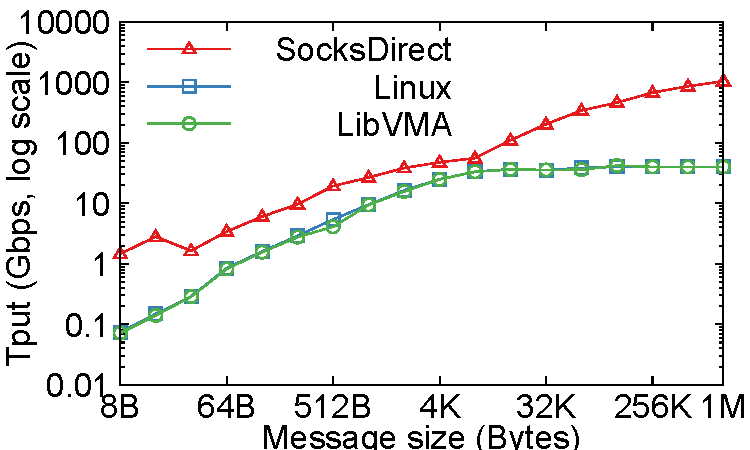
\includegraphics[width=\textwidth]{eval/microbenchmark/msgsize-ipc-tput.pdf}
			\label{fig:eval-msgsize-ipc-tput}
			%\end{minipage}
		}
		\vspace{-10pt}
		\subfloat[intra-host latency]{
			%\begin{minipage}{0.4\textwidth}
			\centering 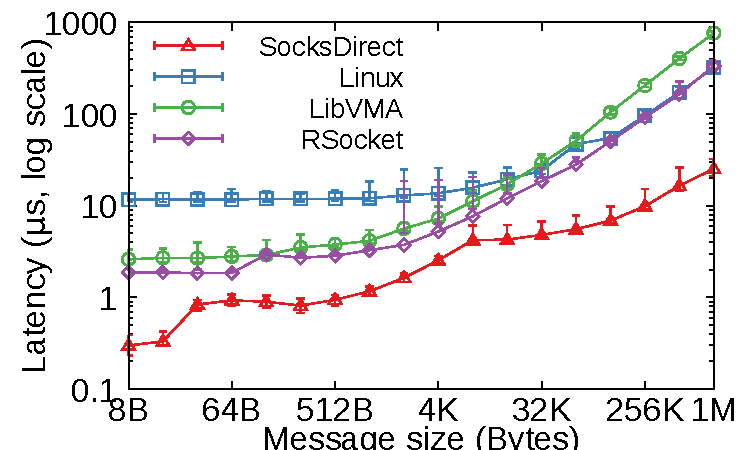
\includegraphics[width=\textwidth]{eval/microbenchmark/msgsize-ipc-lat.pdf}
			\label{fig:eval-msgsize-ipc-lat}
			%\end{minipage}
		}
		\vspace{-10pt}
		\caption{Single-core intra-host performance with message sizes.}
		\label{fig:eval-msgsize-intra}
	\end{minipage}
	\hspace{0.01\textwidth}
	\begin{minipage}{.31\textwidth}
		\centering
		\subfloat[inter-host throughput]{
			%\begin{minipage}{0.4\textwidth}
			\centering 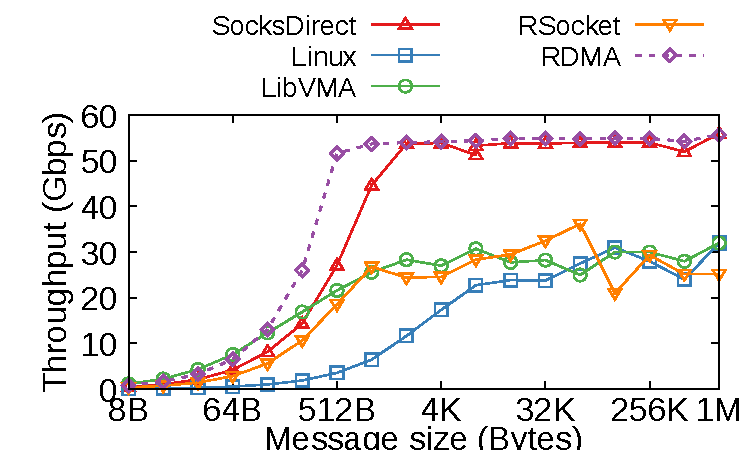
\includegraphics[width=\textwidth]{eval/microbenchmark/msgsize-network-tput.pdf}
			\label{fig:eval-msgsize-network-tput}
			%\end{minipage}
		}
		\vspace{-10pt}
		\subfloat[inter-host latency]{
			%\begin{minipage}{0.4\textwidth}
			\centering 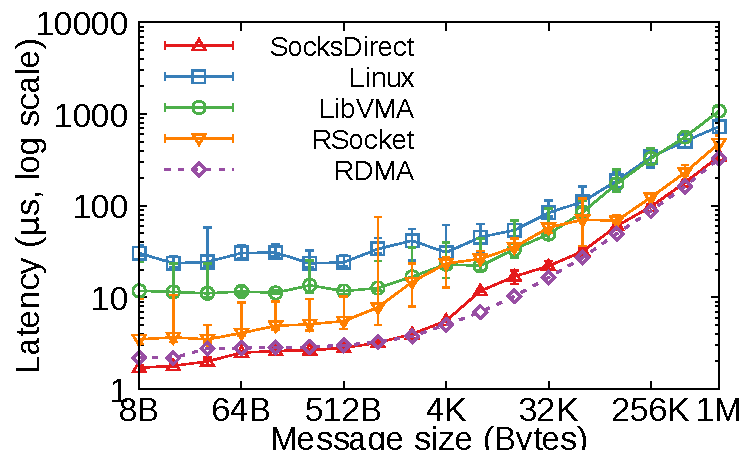
\includegraphics[width=\textwidth]{eval/microbenchmark/msgsize-network-lat.pdf}
			\label{fig:eval-msgsize-network-lat}
			%\end{minipage}
		}
		\vspace{-10pt}
		\caption{Single-core inter-host performance with message sizes.}
		\label{fig:eval-msgsize-inter}
	\end{minipage}
	\hspace{0.01\textwidth}
	\begin{minipage}{.31\textwidth}
		\subfloat[intra-host]{                    
			%\begin{minipage}{0.4\textwidth}
			\centering
			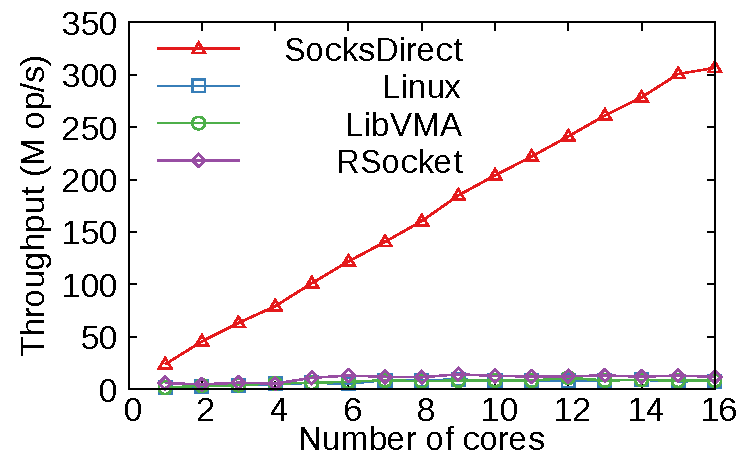
\includegraphics[width=\textwidth]{eval/microbenchmark/corenum-IPC-tput.pdf}
			\label{fig:eval-cornum-ipc}
			%\end{minipage}
		}
		\vspace{-5pt}
		\subfloat[inter-host]{
			%\begin{minipage}{0.4\textwidth}
			\centering 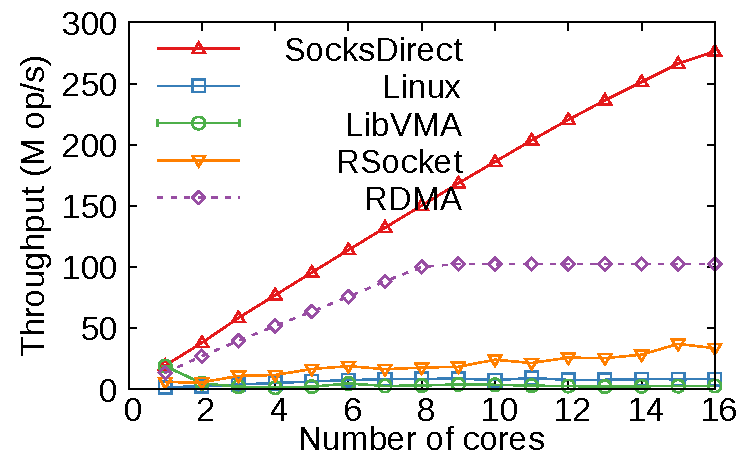
\includegraphics[width=\textwidth]{eval/microbenchmark/corenum-network-tput.pdf}
			\label{fig:eval-cornum-network}
			%\end{minipage}
		}
		\vspace{-10pt}
		\caption{8-byte data transmission throughput with number of cores.}
		\label{fig:eval-corenum-tput}
	\end{minipage}
	\iffalse
	\begin{minipage}{.31\textwidth}
		\centering
		\subfloat[intra-host]{                    
			%\begin{minipage}{0.4\textwidth}
			\centering
			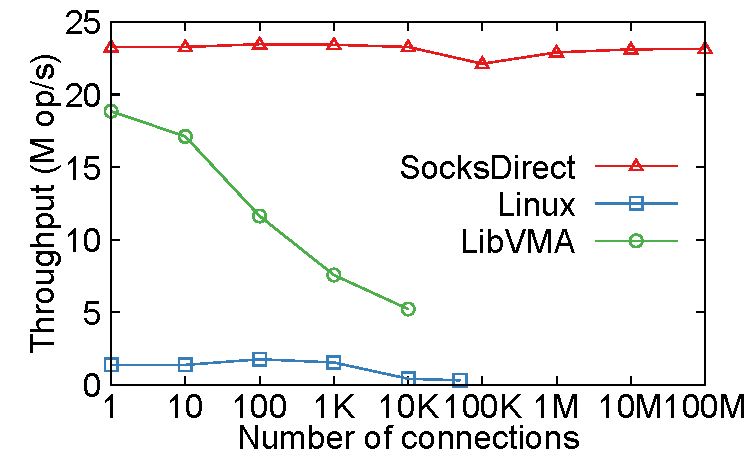
\includegraphics[width=\textwidth]{eval/microbenchmark/connnum-ipc-tput.pdf}
			\label{fig:eval-connnum-ipc-tput}
			%\end{minipage}
		}
		\vspace{-10pt}
		\subfloat[inter-host]{
			%\begin{minipage}{0.4\textwidth}
			\centering 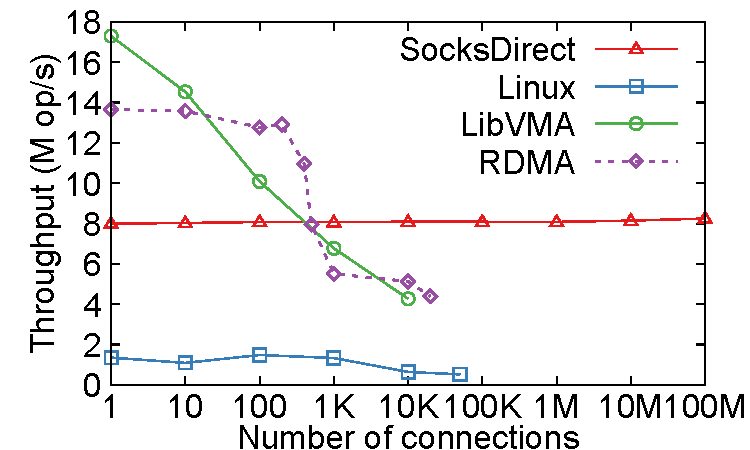
\includegraphics[width=\textwidth]{eval/microbenchmark/connnum-network-tput.pdf}
			\label{fig:eval-connnum-network-tput}
			%\end{minipage}
		}
		\vspace{-5pt}
		\caption{Single-core throughput with number of connections.}
		\label{fig:eval-connnum-tput}
	\end{minipage}
	\fi
	\vspace{-15pt}
\end{figure*}

%\begin{figure}[htpb]
%	\centering
%	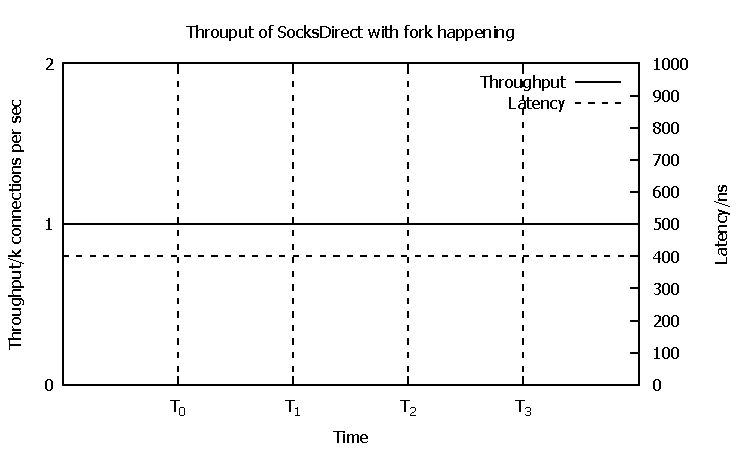
\includegraphics[width=\columnwidth]{eval/microbenchmark/fork-tput.pdf}
%	\caption{Throughput of SocksDirect with fork happening}
%	\label{fig:eval-fork-tput}
%\end{figure}

We implement \sys in three components: a user-space library \libipc{} and a monitor daemon with 17K lines of C++ code, and a modified RDMA NIC driver to support zero copy. We evaluate \sys in the following aspects:

\parab{Use shared memory efficiently for intra-host socket.}
For small messages, \sys achieves 0.3$\mu$s round-trip latency and up to 23~M messages per second throughput, close to raw SHM performance. For large messages, \sys uses zero copy to achieve 1/13 latency and 26x throughput than Linux.

\parab{Use RDMA efficiently for inter-host socket.}
\sys achieves 1.7$\mu$s round-trip latency and 18M messages per second throughput, close to raw RDMA performance.

%\parab{Robust with number of connections.}
%The performance above can be maintained with up to 100 million connections.

\parab{Scale with number of cores.}
The performance above is linearly scalable with number of cores. %In addition, a single CPU core can create 1.4~M connections per second.

%\parab{Corner-case operations does not affect long-term performance.}
%After corner-case operations such as \texttt{fork}, the performance recovers quickly.

\parab{Significant speedup with unmodified real-world applications.}
\sys{} is compatible with many real-world applications.
It achieves 5.5x latency reduction for Nginx, Redis and ZeroMQ.
It also improves throughput of a network function chain by 15x.


\subsection{Methodology}
\label{subsec:methodology}

We evaluate \sys on servers with two Xeon E5-2698 v3 CPUs, 256~GiB memory and a Mellanox ConnectX-4 NIC. The servers are interconnected with an Arista 7060CX-32S 100G switch~\cite{arista-7060cx}. We use Ubuntu 16.04 with Linux 4.15, RoCEv2 for RDMA and poll completion queue every 64 messages.
Each thread is pinned on a CPU core. We run tests for enough warm-up rounds before collecting data.
For latency, we build a ping-pong application and report the mean round-trip time, with error bars representing 1\% and 99\% percentile.
For throughput, one side keeps sending data while the other side keeps receiving data.
We compare with Linux, raw RDMA write verb, Rsocket~\cite{rsockets}, and LibVMA~\cite{libvma}, a user-space TCP/IP stack optimized for Mellanox NICs.
We did not evaluate mTCP~\cite{jeong2014mtcp} because the underlying DPDK library has limited support on our NIC. mTCP has much higher latency than RDMA due to batching, and the reported throughput was 1.7~M packets per second~\cite{kalia2018datacenter}. %The throughput reported in mTCP paper was 1.7~M packets per second~\cite{kalia2018datacenter}, while RDMA achieves more than 10~M messages per second.
This work does not raise any ethical issues.

\subsection{Microbenchmarks}
\label{subsec:microbenchmark}

\subsubsection{Latency and Throughput}
\quad



Figure~\ref{fig:eval-msgsize-intra} shows intra-host socket performance between a pair of sender and receiver threads.
For 8-byte messages, \sys achieves 0.3$\mu$s round-trip latency (1/35 of Linux) and 23~M messages per second throughput (20x of Linux).
In comparison, a simple SHM queue has 0.25$\mu$s round trip latency and 27~M throughput, indicating that \sys adds little overhead.
RSocket has 6x latency and 1/4 throughput of \sys{}, because it uses the NIC to forward intra-host packets, which incurs PCIe latency.
LibVMA simply uses kernel TCP socket for intra-host.
The one-way delay of \sys{} is 0.15$\mu$s, even lower than a kernel crossing (0.2$\mu$s). Kernel-based sockets require a kernel crossing on both sender and receiver.

Due to memory copy, for 8~KiB messages, the throughput of \sys is only 60\% higher than Linux, and the latency is 4x lower. For messages with at least 16~KiB size, \sys uses page remapping to achieve zero copy.
For 1~MiB messages, \sys achieves 1/13 latency and 26x throughput than Linux.
The latency of RSocket is unstable and may be even larger than Linux in some cases, because of event notification delay.


Figure~\ref{fig:eval-msgsize-inter} shows inter-host socket performance between a pair of threads.
For 8-byte messages, \sys achieves 18M messages per second throughput (15x of Linux) and 1.7$\mu$s latency (1/17 of Linux).
The throughput and latency is close to raw RDMA write operations (shown as dashed line), which does not have socket semantics.
\sys{} has even higher throughput than RDMA for 8-byte messages due to batching.
LibVMA also uses batching to achieve better throughput than \sys{} for 16 to 128 byte messages, but the latency is 7x of \sys{}.
For message sizes less than 8~KiB, the throughput of inter-host RDMA is  slightly lower than intra-host SHM, because the ring buffer structure is shared.
For 512B to 8KiB messages, \sys{} is bounded by packet copy, but still faster than RSocket and LibVMA due to reduced buffer management overheads.
For zero copy messages ($\ge$16 KiB), \sys{} saturates the network bandwidth, which has 3.5x throughput of all compared works and 72\% latency of RSocket.



\begin{figure*}[t!]
	\centering

	\hspace{0.01\textwidth}
	\begin{minipage}{.31\textwidth}
		%\centering
		%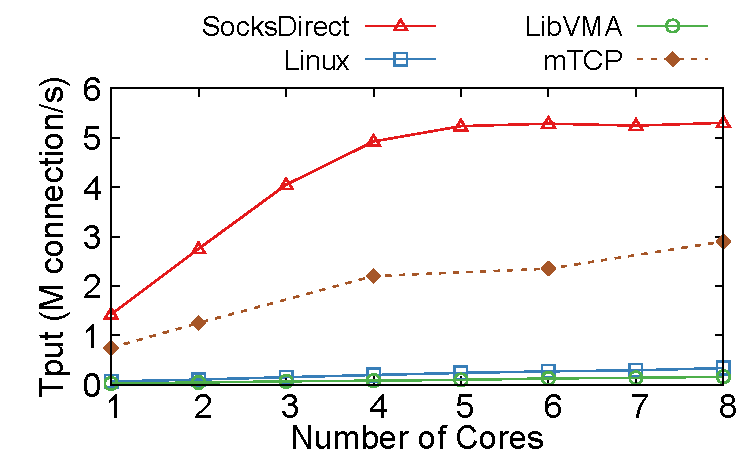
\includegraphics[width=\textwidth]{eval/microbenchmark/conn-setup-tput.pdf}
		%\vspace{-10pt}
		%\caption{Connection creation throughput with number of cores.}
		%\label{fig:eval-conn-setup-tput}
		
		%\begin{minipage}{0.4\textwidth}
		\centering 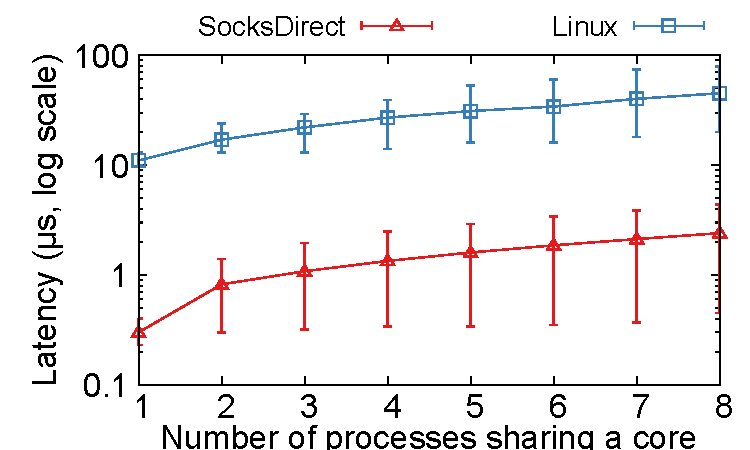
\includegraphics[width=\textwidth]{eval/microbenchmark/sharecore-lat.pdf}
		\vspace{-15pt}
		\caption{Message processing latency where processes share a core.}
		\label{fig:eval-context-switch}
		%\end{minipage}
	\end{minipage}
	\hspace{0.01\textwidth}
	\begin{minipage}{.31\textwidth}
		\centering
		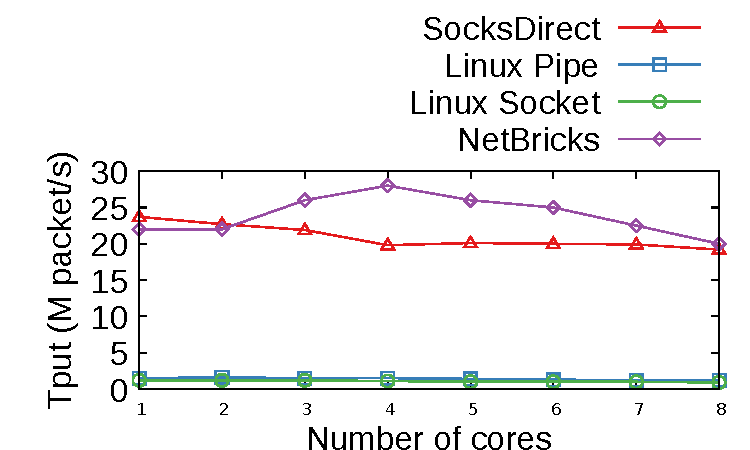
\includegraphics[width=\textwidth]{eval/microbenchmark/nfv-tun-tput.pdf}
		\vspace{-15pt}
		\caption{Throughput of network function pipeline.}
		\label{fig:eval-tun-tput}
		%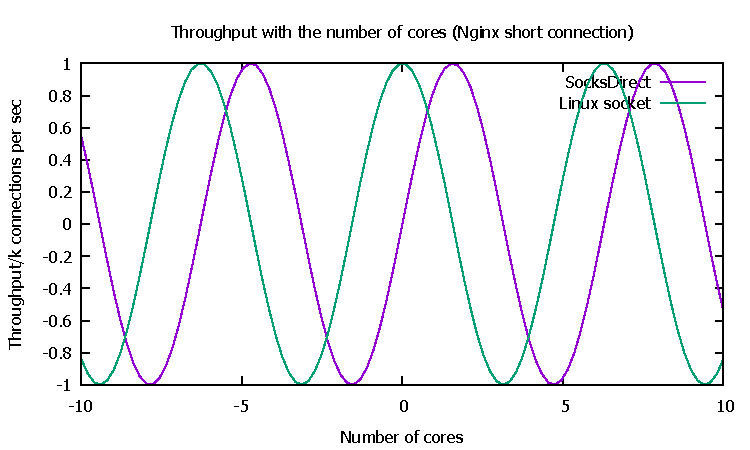
\includegraphics[width=\textwidth]{eval/microbenchmark/nginx-short-tput.pdf}
		%\vspace{-15pt}
		%\label{fig:eval-nginx-short}
		%\caption{Nginx throughput.}
		
		%\centering 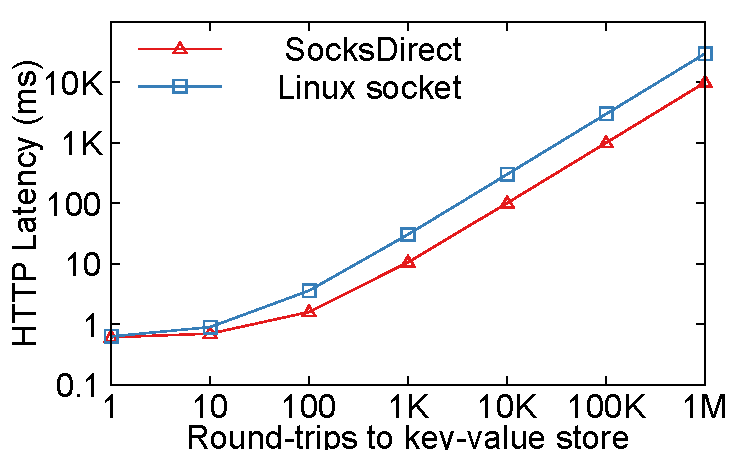
\includegraphics[width=\textwidth]{eval/microbenchmark/nginx-multiround-tput.pdf}
		%\vspace{-15pt}
		%\caption{End-to-end HTTP request latency of a web service.}
		%\label{fig:eval-nginx-multiround}
		
		%\centering
		%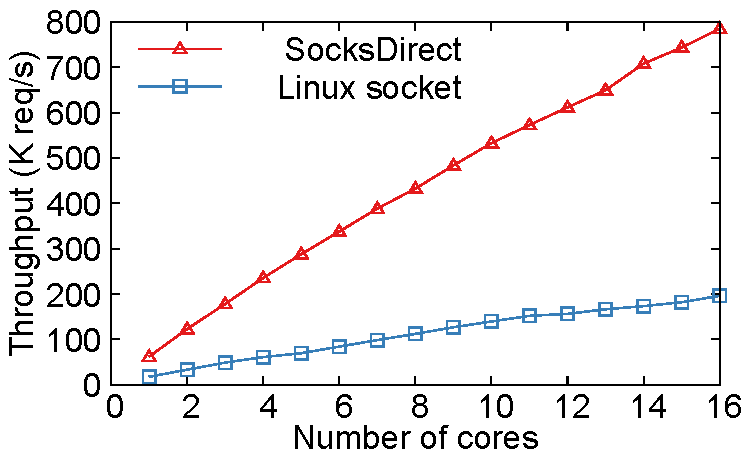
\includegraphics[width=\textwidth]{eval/microbenchmark/corenum-http-tput.pdf}
		%\vspace{-15pt}
		%\caption{Multi-core scalability of HTTP backend service throughput.}
		%\label{fig:eval-http-tput}
	\end{minipage}
	\vspace{-15pt}
\end{figure*}

\subsubsection{Multi-core Scalability}
\quad

%Figure~\ref{fig:eval-connnum-tput} shows the throughput with different number of concurrent connections.
%We establish connections between two processes before testing, then send and receive data from the connections in a round-robin order.
%\sys can support more than 100 million concurrent connections with 16~GiB of memory, and the throughput does not degrade under such high concurrency.
%\sys achieves connection stability by multiplexing connections via a single queue.
%In comparison, the performance of RDMA, LibVMA and Linux drops quickly as the number of connections increase. There is a sharp performance drop with more than 512 RDMA connections, because the RDMA transport states saturate the NIC cache. Although LibVMA and Linux do not use RDMA as transport, they maintain per-FD buffers, which lead to CPU cache and TLB miss with thousands of connections. Furthermore, LibVMA installs flow steering rules to NIC for each connection, which also leads to NIC cache miss.




Figure~\ref{fig:eval-corenum-tput} shows the throughput of 8-byte messages with different number of cores.
Sender and receiver process each creates several threads, then each thread pins on a core and communicates with a peer thread.
\sys achieves almost linear scalability for both intra-host and inter-host sockets.
For intra-host socket, \sys provides 306~M message per second throughput between 16 pairs of sender and receiver cores, which is 40x of Linux and 30x of RSocket.
LibVMA falls back to Linux for intra-host socket.
Using RDMA for inter-host socket, \sys uses batching to achieve 276~M messages per second throughput with 16 cores, which is 2.5x of the message throughput of our RDMA NIC.
RSocket peeks at 24~M for intra-host and 33~M for inter-host due to limited scalability of buffer management.
%Although \sys{} creates $n^2$ queues for $n$ sender and receiver threads, in this workload only $n$ of them are active.
%Because the NIC only caches active RDMA connections and \libipc{} only polls active queues, the idle queues do not degrade performance.
Due to lock contention on shared NIC queues, compared to single thread, the throughput of LibVMA reduces to 1/4 with two threads, and 1/10 with three and more threads.
The Linux throughput scales linearly from 1 to 7 cores and bottlenecks on the loopback or NIC queues with more cores.
%The multi-thread scalability of \sys attributes to the partitioning of states and removal of synchronization.
%We can also see that shared memory communication has 5x throughput than RDMA.% Using RDMA NIC for intra-host socket would meet this bottleneck and thus not scalable.

%Figure~\ref{fig:eval-conn-setup-tput} shows the throughput of connection creation with different number of cores. Each core can create 1.4~M new connections per second, which is 20x of Linux and 2x of mTCP~\cite{jeong2014mtcp}. The upper bound is 5.3~M connections per second, where the monitor becomes a bottleneck.


Finally, we evaluate the performance of multiple threads sharing a core. Each thread needs to wait for its turn to process messages.
As Figure~\ref{fig:eval-context-switch} shows, although the message processing latency increases almost linearly with number of active processes, it is still 1/20 to 1/30 of Linux.



%Finally, we benchmark the throughput and latency after \texttt{fork} and other corner-case operations. Initially, there is only one pair of sender and receiver. At time $T_0$, receiver forks, and the parent process keeps receiving. At time $T_1$, the child process begins to receives takes over the socket. At time $T_2$, sender forks, and only the parent sends. At time $T_3$, the child sender also starts sending. We find that both throughput and latency resume to initial maximal performance within 1~ms after each event.

\subsection{Application Performance}
\label{subsec:application}

In this section, we demonstrate that \sys{} can significantly improve the performance of real-world applications without modifying the code.
Rsocket~\cite{rsockets} cannot run the following applications, so we compare the performance with Linux and libvma~\cite{libvma}.

\subsubsection{Nginx HTTP Server}
\quad

We use Nginx~\cite{nginx} HTTP server as reverse proxy between an HTTP request generator and an HTTP response generator.
Each thread of the generators use a persistent TCP connection to communicate with Nginx.

Figure: latency vs request size.

Figure: 1KB request throughput scalability with number of cores.

\subsubsection{Redis Key-Value Store}
\quad

Redis~\cite{redis}

Figure: line chart, y axis: throughput, lines: (intra-, inter-) x (\sys{}, libvma, Linux). x axis: number of concurrent clients.

Utility: redis-benchmark.
Key point: concurrency low: test latency, concurrency high: test throughput.

%\subsection{Real-time Stream Processing}

%Apache Flink~\cite{carbone2015apache} (need to turn off durability on disk)

%Scenario: Word Count (distributed system with one source, two mappers and one reducer)

%Metrics: Latency, throughput

\subsubsection{ZeroMQ Message Queue}
\quad

Figure: line chart, y axis: latency, lines: (intra-, inter-) x (\sys{}, libvma, Linux), x axis: msg size.

Utility: zeromq official test zeromq\_lat.
Key point: latency is low.

\subsubsection{Network Function Chain}
\quad

Each network function is a process that inputs from stdin and outputs to stdout. Standard pcap packet format. use \emph{pipe} to connect. Compare with Linux pipe and state-of-the-art. Figure~\ref{fig:eval-tun-tput}
Key point: intra-host is important.

\subsubsection{GraphX on Spark}
\quad

Two nodes run distributed PageRank.
Test elapsed time per iteration with \sys{}, libvma and Linux. (Only need three numbers, no figure.)
\section{Discussion}
\label{sec:discussion}

There are several scalability problems in using one or more dedicated cores accelerate distributed coordination.
First, when the number of synchronization objects are large, \textit{e.g.}, one lock per record in databases and the access pattern is close to uniformly random, the throughput is bound by random access to non-cached memory, due to limited parallelism in a CPU core~\cite{lim2014mica}.
Second, when one CPU core is not capable to coordinate the requests, synchronization objects are distributed to multiple coordination cores. However, load imbalance may occur for highly contended objects, \textit{e.g.}, sequencers, socket accept queues and locks for extremely popular database entries.
Finally, when networking and synchronization is not the bottleneck, the dedicated cores are still polling, wasting energy and CPU resources.

\section{Related Work}
\label{sec:related}

There has been extensive work aiming to release the bare metal performance of multi-core CPU and data center network. Table~\ref{tab:related-work} categorizes and compares several representative existing approaches.

\parab{Linux kernel optimization.}
One line of research optimize the kernel code for higher socket performance, for example FastSocket~\cite{lin2016scalable}.
First, the kernel optimization approach does not eliminate kernel crossing overhead, while system call batching introduces extra latency.
Second, the socket interface still needs memory copy.
Third, for many concurrent connections, the kernel requires large memory footprint and thus may introduce cache misses.


\parab{New kernel stacks.}
Another line of research propose kernel stacks with new interfaces.
Arrakis~\cite{peter2016arrakis} and IX~\cite{belay2017ix} use NIC for both intra-server and inter-server communications. The hairpin latency from CPU to NIC is at least two PCIe delays, which is roughly 1$\mu$s~\cite{kaminsky2016design}, one order of magnitude higher than inter-core communication delay ($\leq0.1\mu$s). In addition, the data plane switching capacity of a NIC is constrained by PCIe bandwidth, an order of magnitude lower than the bus among CPU cores~\cite{li2017kv}. For inter-server communication, IX~\cite{belay2017ix} implement transport in software, while Arrakis~\cite{peter2016arrakis} offload the transport to NIC. IX~\cite{belay2017ix} and NetKernel~\cite{niu2017network} enforce SLA in the kernel or hypervisor. Although software has more flexibility than the hardware-based transport in NIC, NICs are becoming increasingly programmable, and the architecture of programmable NICs is a better fit for implementing transport protocols~\cite{kaufmann2015flexnic,smartnic,mellanox,cavium}. 
Stackmap~\cite{yasukata2016stackmap} reuses the TCP/IP stack in Linux kernel to achieve protocol compatibility, but the abstraction for applications are changed to support zero copy.

Although these new stacks demonstrate high performance, existing socket applications need modifications to use the new abstractions.
Furthermore, for large scale deployment, kernel-based stacks are much more complicated than user-space libraries~\cite{andromeda}.


%\parab{RDMA.}
%First, RDMA is not suitable for WAN. Second, RDMA has scalability issue when one server connects to many servers. Software transport in CPU access connection states in host memory, while hardware RDMA transport caches connection states in NIC and swaps out to host memory when cache overflows. First, CPU cache miss costs less than 0.1$\mu$s, while NIC cache miss costs 0.5$\mu$s~\cite{kaminsky2016design}. Second, CPU memory bandwidth is an order of magnitude larger than NIC PCIe bandwidth. In light of this, a host should switch to software transport when it actively communicates with a large number of hosts. Fortunately, Modern NICs has an increasing size of memory and supports more active connections without performance degradation~\cite{kaminsky2016design}.




\iffalse
Kernel-bypass TCP/IPs
IX [OSDI’14], Arrakis [OSDI’14], UTCP [CCR’14], Sandstorm [SIGCOMM’14], mTCP [NSDI’14], Seastar

Socket API enhancements
MegaPipe [OSDI’12], FlexSC [OSDI’10], KCM [Linux]

Improving OS stack with fast packet I/O
mSwitch [SOSR’15]

In-stack improvement
FastSocket [ASPLOS’16]

Running kernel stack in user-space
Rump [AsiaBSDCon’09], NUSE [netdev’15]
\fi





%\textbf{User-space socket.}
%mTCP~\cite{jeong2014mtcp}

%SDP~\cite{socketsdirect} and rsockets~\cite{rsockets} are not compatible with Linux socket because the application still needs to manage send and receive buffers.

\iffalse
\begin{itemize}
	\item New abstraction (RDMA, lwip + DPDK etc.) 
	\begin{itemize}
		\item 
	\end{itemize}
	\item Compatible with socket (libvma, LOS etc.) 
	\begin{itemize}
		\item Violate goal 2: memory copy 
		\item Violate goal 3: thread synchronization for multi-thread applications 
	\end{itemize}
	\item Common problems: 
	\begin{itemize}
		\item Designed for networking, does not support or optimize for IPC communication inside the same server 
		\item Violate goal 4: Not optimized for many connections 
	\end{itemize}
\end{itemize}
\fi


\section{Conclusion}
\label{sec:conclusion}

There has been a long debate on where to implement network stacks: hardware, kernel or user-space. With programmable NIC, hardware and software can work together by separation of coordination-intensive control plane and communication-intensive data plane. By offloading some kernel functionalities to hardware as well as user-space, the throughput of short-lived connections and the network delay among containers have an order of magnitude improvement.

A key challenge in FPGA-based NIC design is PCIe latency. With the advent of Xeon+FPGA platform, we expect higher throughput and lower latency communication between CPU and FPGA, to enable more fine-grained hardware-software co-design.

\small 
\balance
\bibliographystyle{abbrv}
\bibliography{reference}

\end{document}
